% Copyright 2023 Fausto Spoto
%
% Licensed under the Apache License, Version 2.0 (the "License");
% you may not use this file except in compliance with the License.
% You may obtain a copy of the License at
%
%    http://www.apache.org/licenses/LICENSE-2.0
%
% Unless required by applicable law or agreed to in writing, software
% distributed under the License is distributed on an "AS IS" BASIS,
% WITHOUT WARRANTIES OR CONDITIONS OF ANY KIND, either express or implied.
% See the License for the specific language governing permissions and
% limitations under the License.

\documentclass[11pt]{beamer}  %% versione proiettore
%%\documentclass[11pt,handout]{beamer} %% versione stampa
\usepackage{lucidiJb-2ed}

\usepackage{mathtools}
\usepackage{relsize}
\usepackage[normalem]{ulem}

\mode<article>
{
  \usepackage{fullpage}
  \usepackage{hyperref}
}

\mode<presentation>
{
  \setbeamertemplate{background canvas}[vertical shading][bottom=red!10,top=blue!10]
  \usetheme{Course}
  \usefonttheme[onlysmall]{structurebold}
}

\subtitle{R\'eunion Island, 13/4/2023}
\title{An Overview of Blockchain Technology}
\institute{Universit\`a di Verona, Italy}
\date{April 2023}

\setbeamercovered{invisible}

\def\codesize{\smaller}
\def\<#1>{\codeid{#1}}
\newcommand{\codeid}[1]{\ifmmode{\mbox{\codesize\ttfamily{#1}}}\else{\codesize\ttfamily #1}\fi}

\AtBeginSection[]{
  \begin{frame}
  \vfill
  \centering
  \begin{beamercolorbox}[sep=8pt,center,shadow=true,rounded=true]{title}
    \usebeamerfont{title}\insertsectionhead\par%
  \end{beamercolorbox}
  \vfill
  \end{frame}
}

\begin{document}

\begin{frame}
  \titlepage
\end{frame}

\begin{frame}
  \tableofcontents
\end{frame}

\section{Introduction}

\begin{frame}\frametitle{The mainstream view of blockchain}

  \begin{center}
    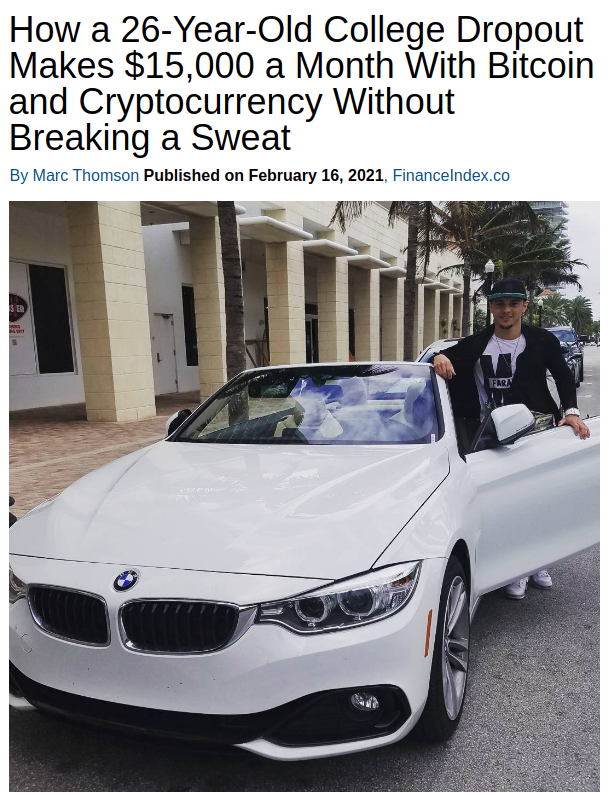
\includegraphics[scale=0.209,clip=false]{pictures/dropout.png}
    \hspace*{2ex}
    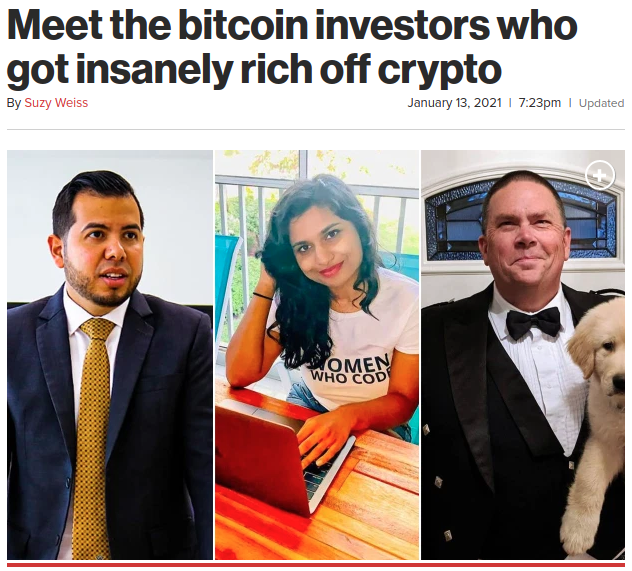
\includegraphics[scale=0.29,clip=false]{pictures/insane.png}
  \end{center}

\end{frame}

\begin{frame}\frametitle{History}

  \begin{itemize}
  \item[1988] proof of work (Dwork \& Naor)
  \item[1991] a cryptographically secure chain of blocks (Haber \& Stornetta)
  \item[199x] smart contracts (Szabo)
  \item[2008] Bitcoin (Nakamoto)
  \item[2012] proof of stake (Peercoin)
  \item[2013] Ethereum (Buterin \& Wood)
  \item[2014] proof of space (Burstcoin/Signum)
  \item[2014] Tendermint generic proof of stake engine (Kwon)
  \item[2022] Ethereum 2.0 moves to proof of stake
  \end{itemize}
  
\end{frame}

\begin{frame}\frametitle{Distributed network}

  \begin{center}
    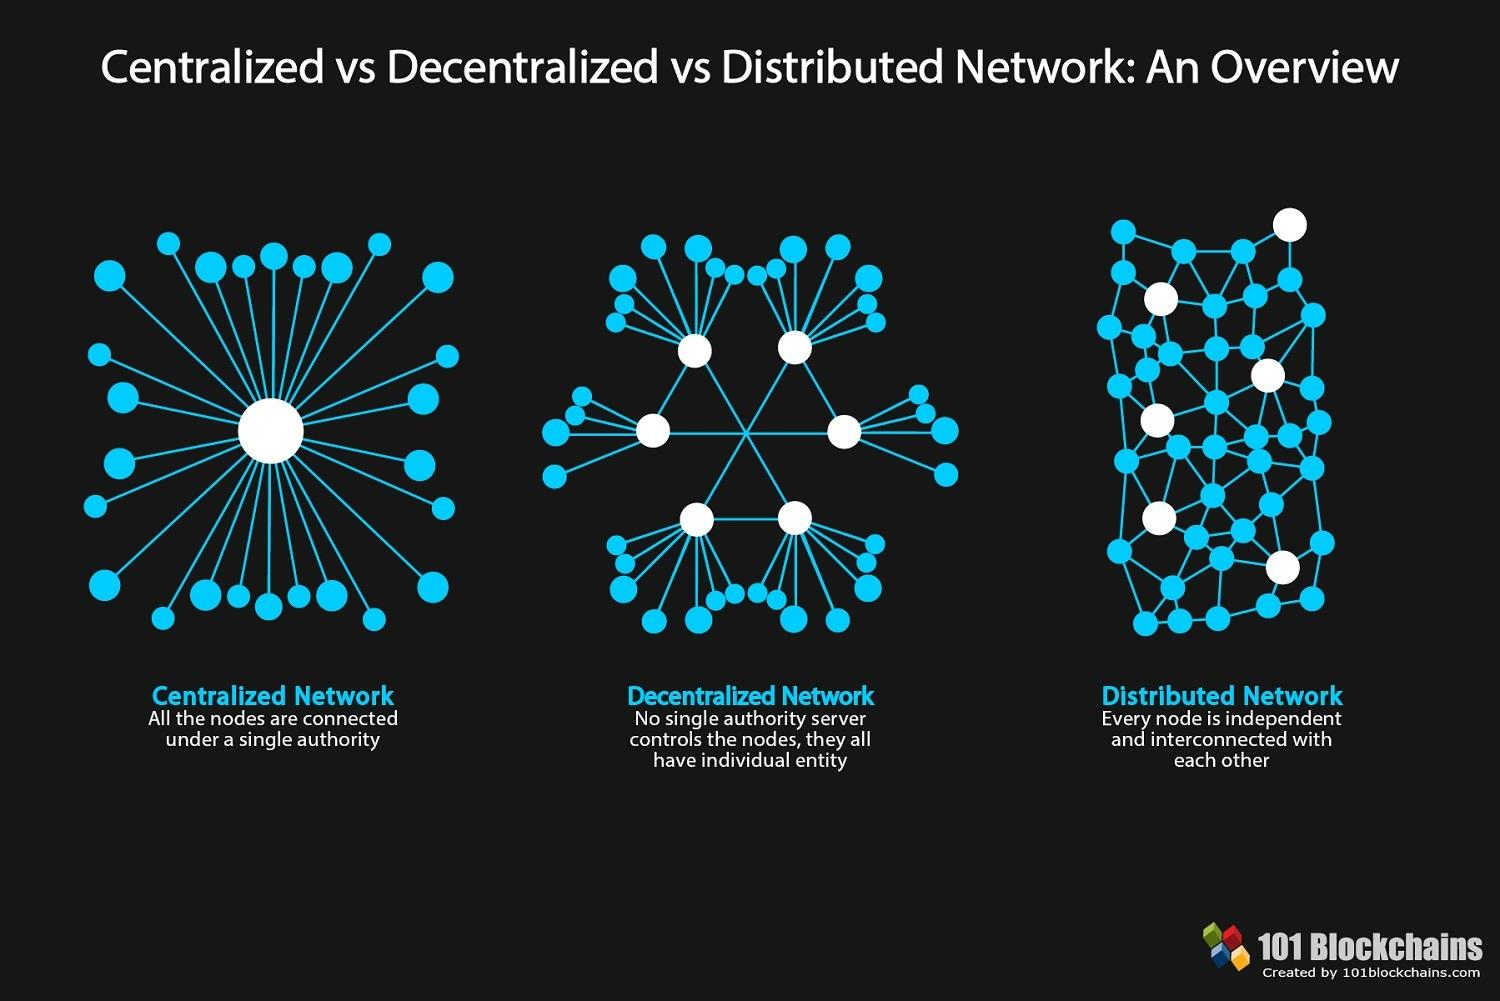
\includegraphics[scale=0.22,clip=false]{pictures/distributed.jpg}
  \end{center}

\end{frame}

\begin{frame}\frametitle{Cryptocurrencies}

  \begin{center}
    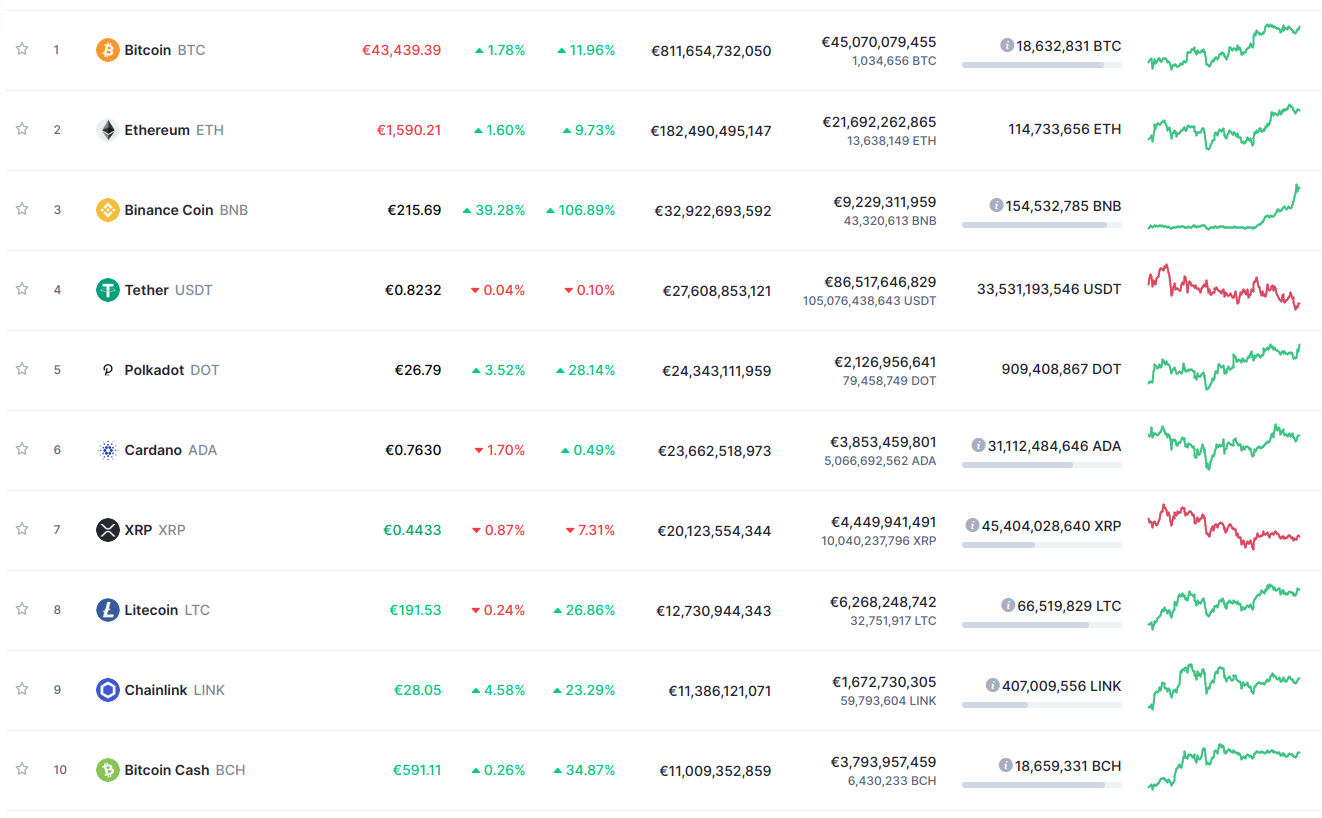
\includegraphics[scale=0.258,clip=false]{pictures/market.png}
  \end{center}

\end{frame}

\begin{frame}\frametitle{Bitcoin chart}

  \begin{center}
    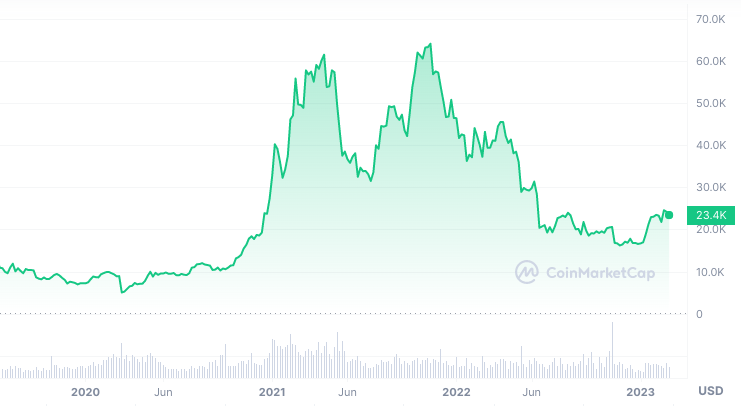
\includegraphics[width=\textwidth,clip=false]{pictures/bitcoin-coinmarketcap.png}
  \end{center}

\end{frame}

\begin{frame}\frametitle{Bitcoin capitalization (2018)}

  \begin{center}
    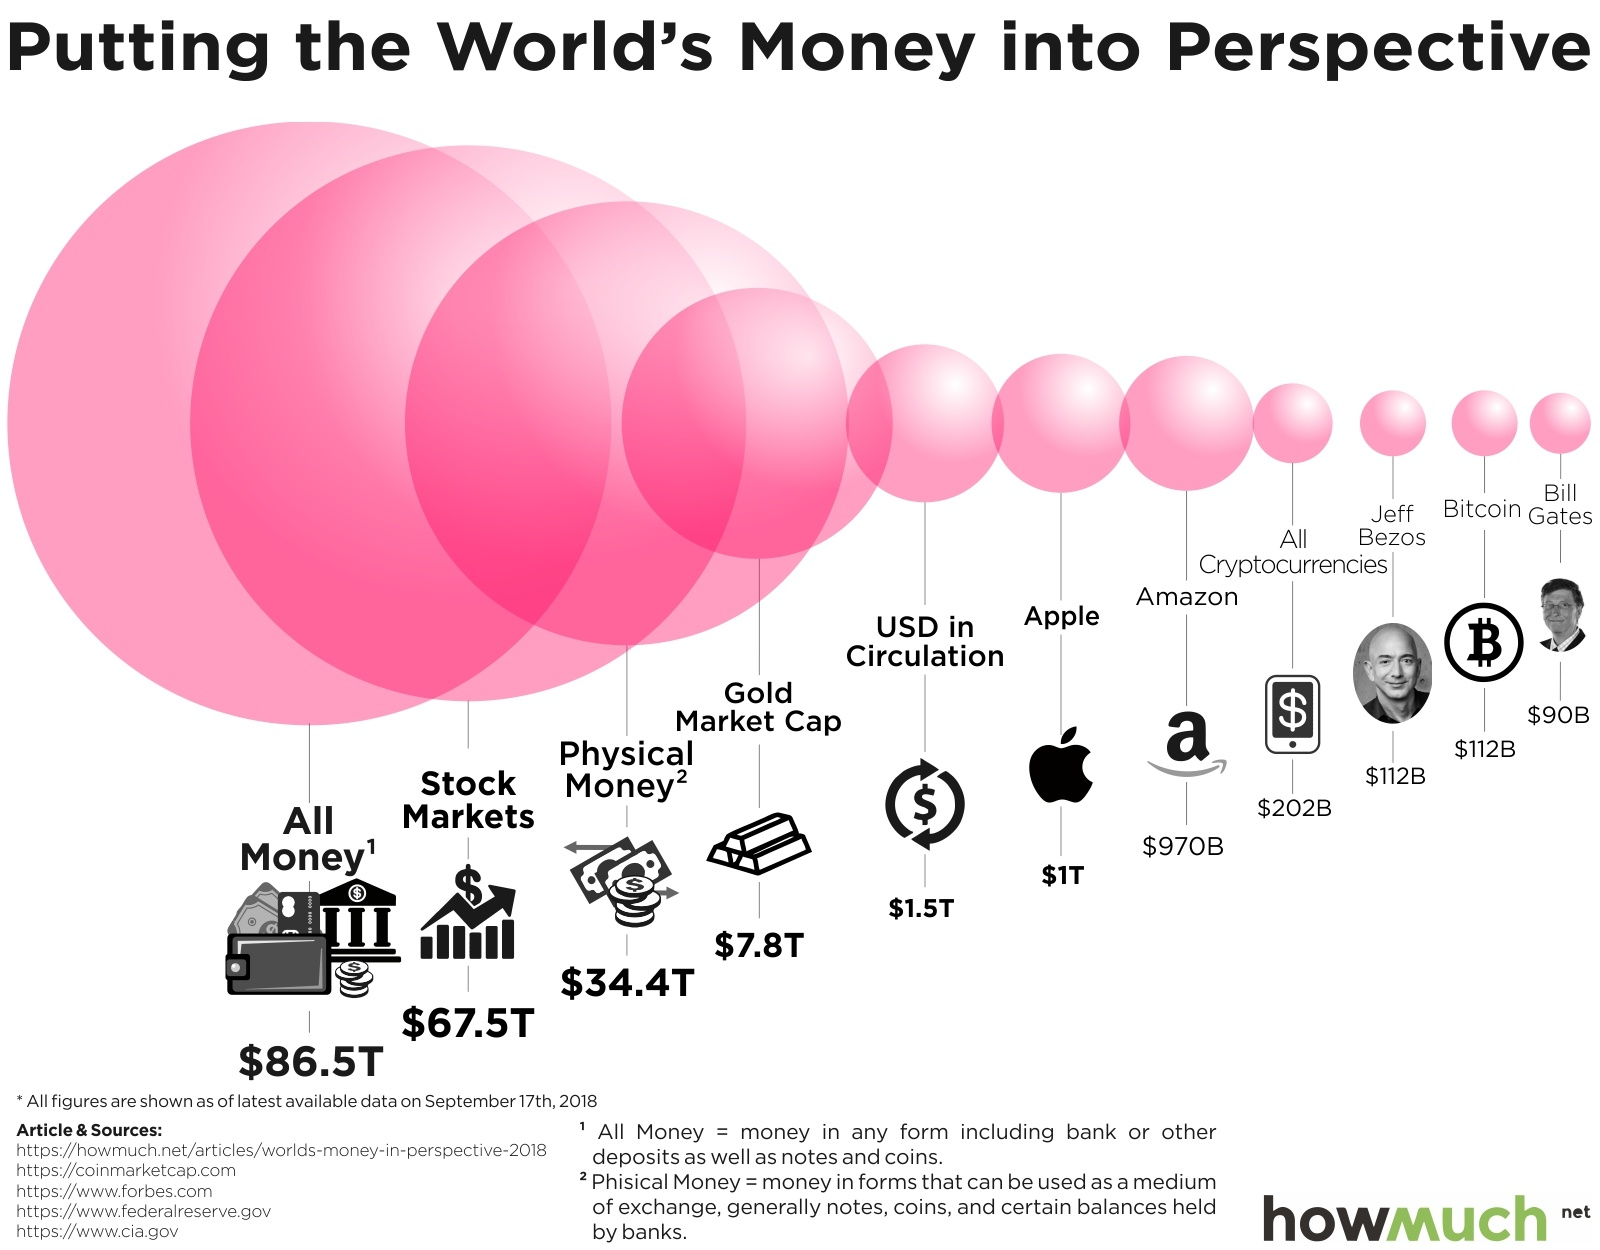
\includegraphics[scale=0.16,clip=false]{pictures/bitcoin-capitalization.jpg}
  \end{center}

  \begin{center}
    source: \url{HowMuch.net}, a financial literacy website
  \end{center}

\end{frame}

\begin{frame}\frametitle{Credit cards transactions (billions, 2018) vs Bitcoin}

  \begin{center}
    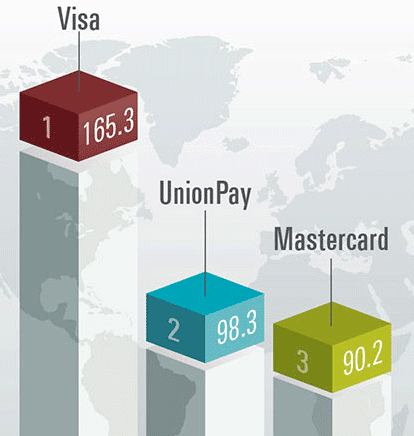
\includegraphics[scale=0.3,clip=false]{pictures/credit-cards.png}
  \end{center}

  \begin{center}
    Visa: around 451,639,000 transactions per day\\
    UnionPay: around 268,579,000 transactions per day\\
    Mastercard: around 246,448,000 transactions per day\\
    Bitcoin: around 300,000 transactions per day
  \end{center}

\end{frame}

\begin{frame}\frametitle{Bitcoin transaction fees}

  \begin{center}
    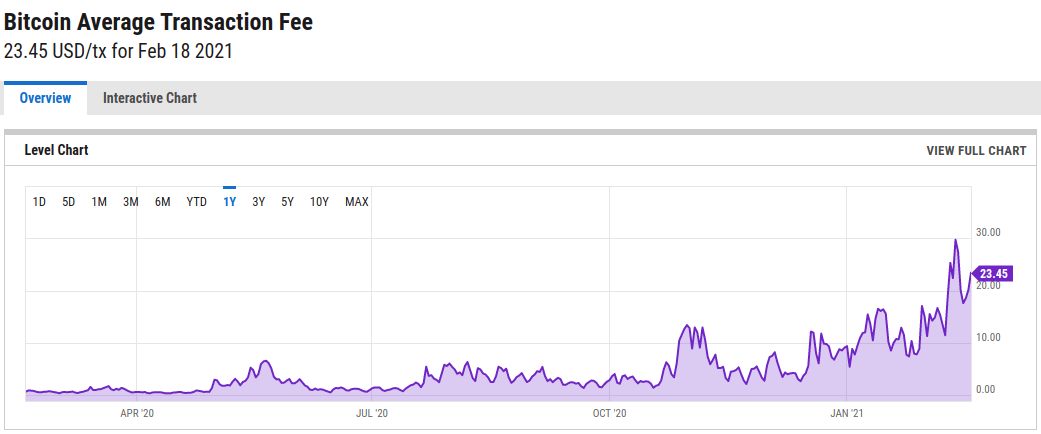
\includegraphics[width=\textwidth,clip=false]{pictures/bitcoin-fees.png}
  \end{center}

  \begin{center}
    Independent from the transacted value
  \end{center}

\end{frame}

\begin{frame}\frametitle{Credit cards transaction fees}

  \begin{center}
    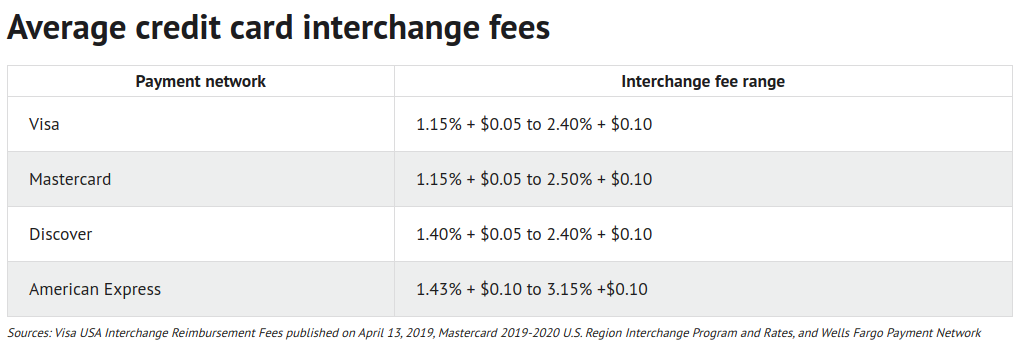
\includegraphics[width=\textwidth,clip=false]{pictures/credit-cards-fees.png}
  \end{center}

  \begin{center}
    Proportional to the transacted value
  \end{center}

\end{frame}

\begin{frame}\frametitle{The hype cycle}

  \begin{center}
    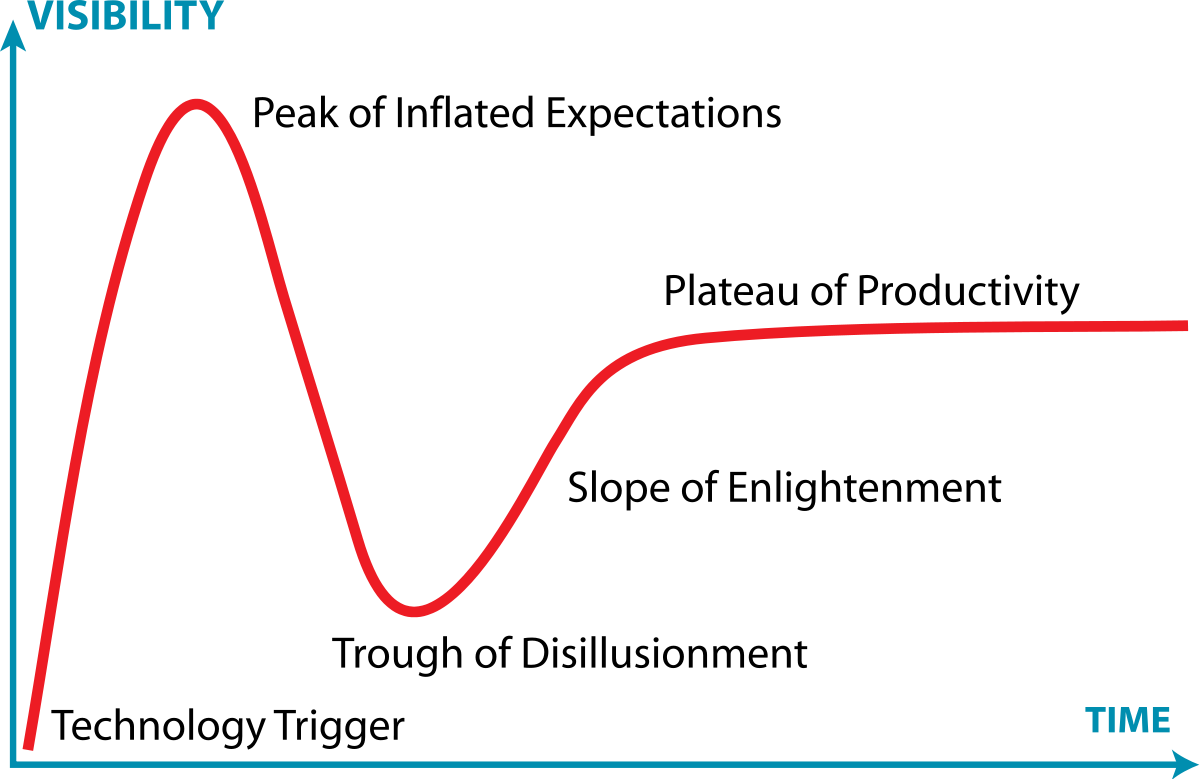
\includegraphics[width=\textwidth,clip=false]{pictures/hype-cycle.png}
  \end{center}

\end{frame}

\begin{frame}\frametitle{Beyond the hype}

  \begin{center}
    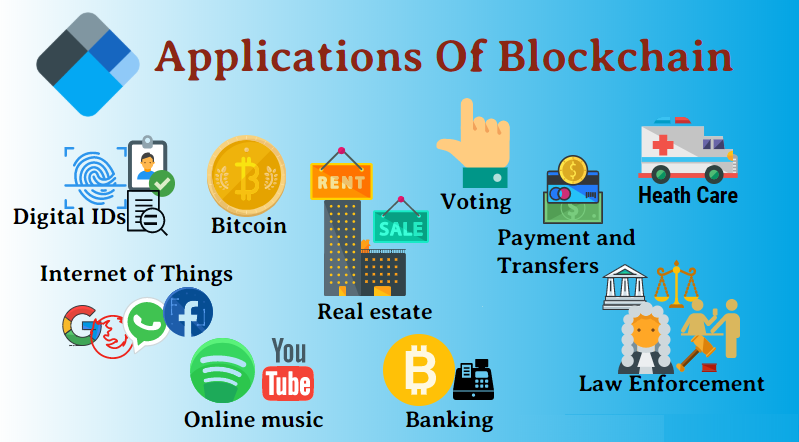
\includegraphics[scale=0.4,clip=false]{pictures/blockchain-applications.png}
  \end{center}

\end{frame}

\section{Bitcoin}

\begin{frame}
  \frametitle{The internet of money}

  \begin{greenbox}{What we expect from money}
    \begin{itemize}
    \item money should be protected from counterfeiting (\emph{legality})
    \item money should not be spent twice (\emph{uniqueness})
    \item no one can claim that my money belongs to him (\emph{ownership})
    \item money should be untained (\emph{fungibility})
    \item money should be movable (\emph{liquidity})
    \end{itemize}
  \end{greenbox}

  \bigskip

  Electronic money exists since decades (credit cards, online transactions)

  \bigskip

  \begin{greenbox}{}
    Bitcoin provides a \alert{fully decentralized} electronic cash system, for the first time
    (a single State cannot shut down the bitcoin network)
  \end{greenbox}

  \bigskip

  ``Bitcoin: A Peer-to-Peer Electronic Cash System'' by Satoshi Nakamoto, 2008

\end{frame}

\begin{frame}\frametitle{The best reference}

  \begin{center}
    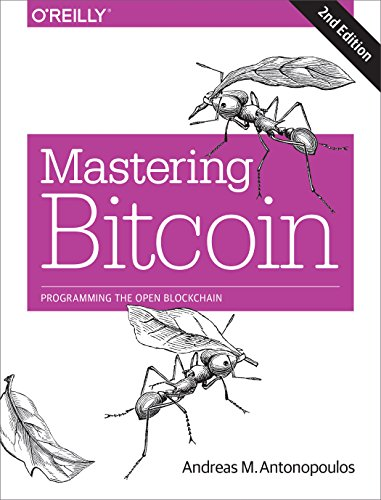
\includegraphics[scale=.35,clip=false]{pictures/mastering-bitcoin.jpg}
  \end{center}

  \begin{center}
    \url{https://github.com/bitcoinbook/bitcoinbook}
  \end{center}

\end{frame}

\begin{frame}\frametitle{Bitcoin as a web service}

  \begin{center}
    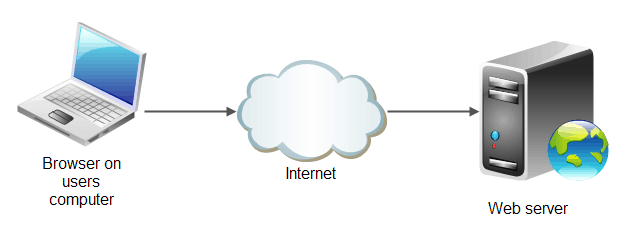
\includegraphics[scale=.3,clip=false]{pictures/web-server.png}
  \end{center}

  \medskip

  The server keeps a map (\alert{ledger}) $\mathit{user\_id}\Rightarrow\mathit{balance}$
  and accepts transactions to transfer balances

  \medskip

  Users interact through a browser (\alert{wallet}) to ask to transfer balances

  \medskip
  The server is actually a worldwide peer-to-peer (p2p) network of computers

  \begin{center}
    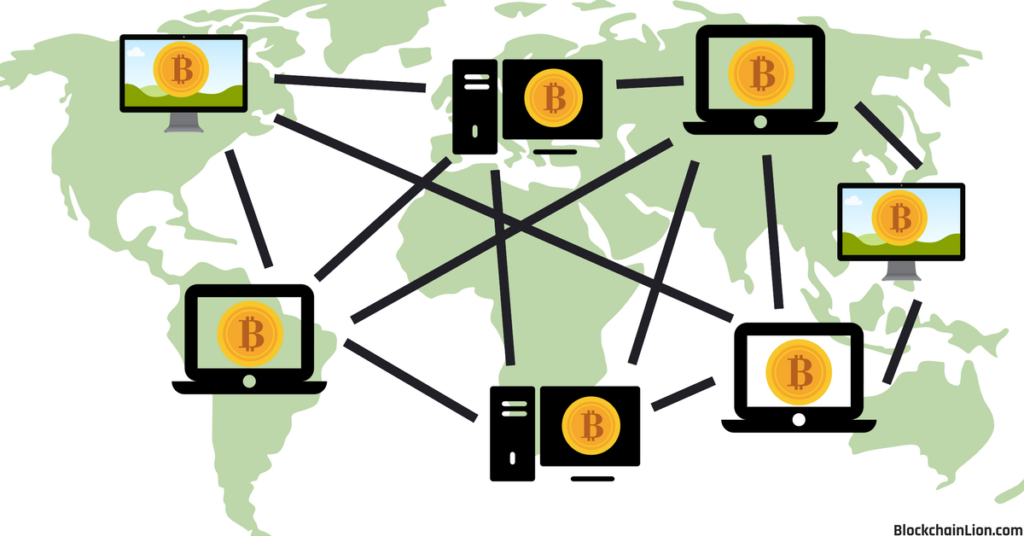
\includegraphics[scale=.13,clip=false]{pictures/distributed.png}
  \end{center}

\end{frame}

\begin{frame}\frametitle{Mobile wallets}

  At the first start-up, a bitcoin address is created for you, then transactions
  from/to that address are tracked:

  \begin{center}
    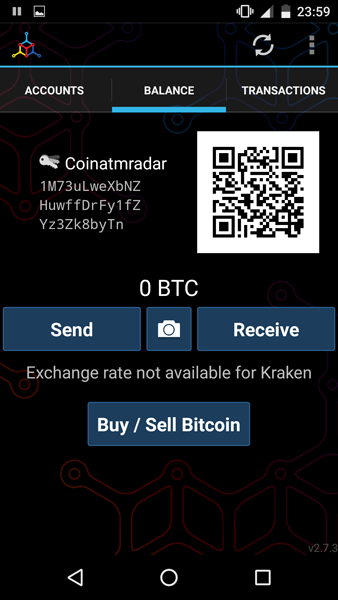
\includegraphics[scale=0.27,clip=false]{pictures/bitcoin-wallet.png}
  \end{center}

  The \alert{address} can be seen as our IBAN. Its creation
  is a local operation that does not do anything on the network: fully anonymous

\end{frame}

\begin{frame}\frametitle{Address creation}

  When Alice's wallet starts for the first time:

  \begin{enumerate}
  \item it generates a finite sequence of bits through a secure random generator
    (a secret private key)
  \item it computes the bitcoin address as an abstraction of the private key
    (hashing)
  \item it shows the bitcoin address as an alphanumeric string and as a picture (QR code)
  \item \alert{the address is not sensitive information}: Alice can publish it in her web page
  \item \alert{the private key is sensitive information}: Alice keeps it secret
    \begin{itemize}
    \item a hardware wallet stores it in its internal memory
    \item a desktop wallet stores it in Alice's computer's file system (!)
    \item a mobile wallet stores it in Alice's phone (!!!)
    \item a web wallet stores it at a third-party service (!!!!!!!)
    \end{itemize}
  \end{enumerate}
\end{frame}

\begin{frame}\frametitle{Alice charges her wallet with a transaction}
  \begin{itemize}
  \item she asks a friend to send bitcoins to her address
  \item meets a bitcoin seller in person
  \item earns bitcoin by working
  \item uses a bitcoin ATM
  \item uses a bitcoin currency exchange company
  \end{itemize}

  \bigskip

  \begin{greenbox}{What is the price?}
    It is not set by the computer network! It's a social
    agreement, the average of the last sell operations.
    You can look online for it
  \end{greenbox}

\end{frame}

\begin{frame}\frametitle{Transactions form a chain, outputs can be change}

  \begin{center}
    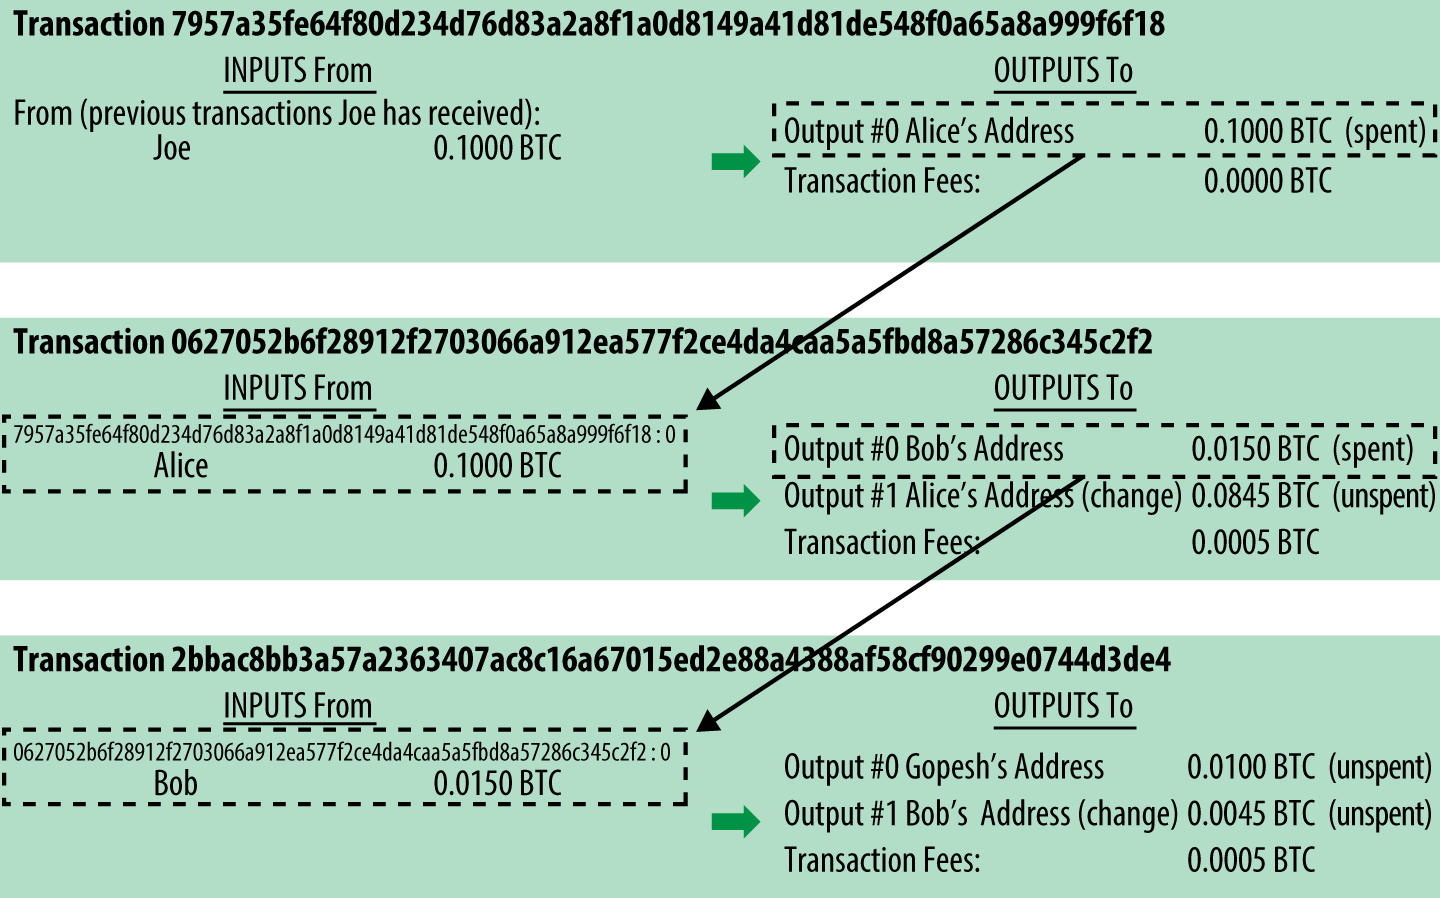
\includegraphics[scale=0.23,clip=false]{pictures/mbc2_0204.png}
  \end{center}

\end{frame}

\begin{frame}\frametitle{Typical transaction: pay somebody and gets the change}

  \begin{center}
    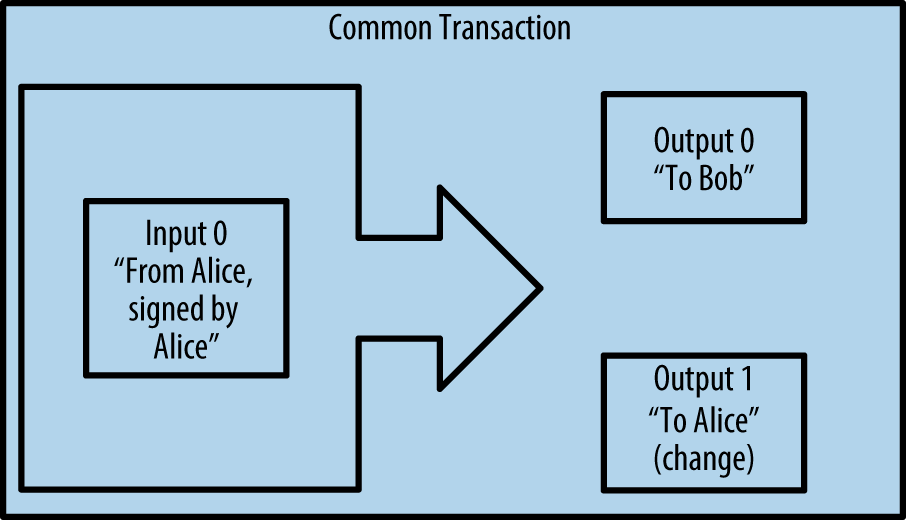
\includegraphics[scale=1.2,clip=false]{pictures/mbc2_0205.png}
  \end{center}

\end{frame}

\begin{frame}\frametitle{Typical transaction: aggregate small notes into a larger one}

  \begin{center}
    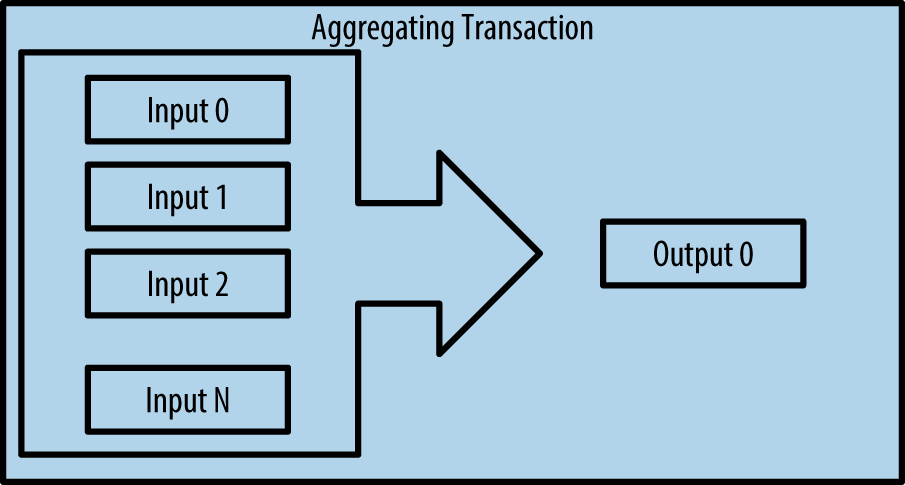
\includegraphics[scale=1.2,clip=false]{pictures/mbc2_0206.png}
  \end{center}

\end{frame}

\begin{frame}\frametitle{Typical transaction: distribution}

  \begin{center}
    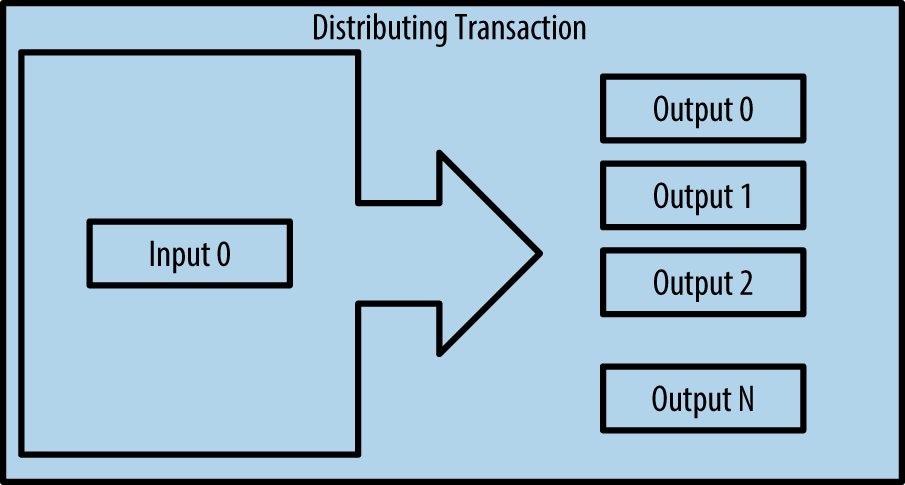
\includegraphics[scale=1.2,clip=false]{pictures/mbc2_0207.png}
  \end{center}

\end{frame}

\begin{frame}\frametitle{A DAG of transactions}

  \begin{center}
    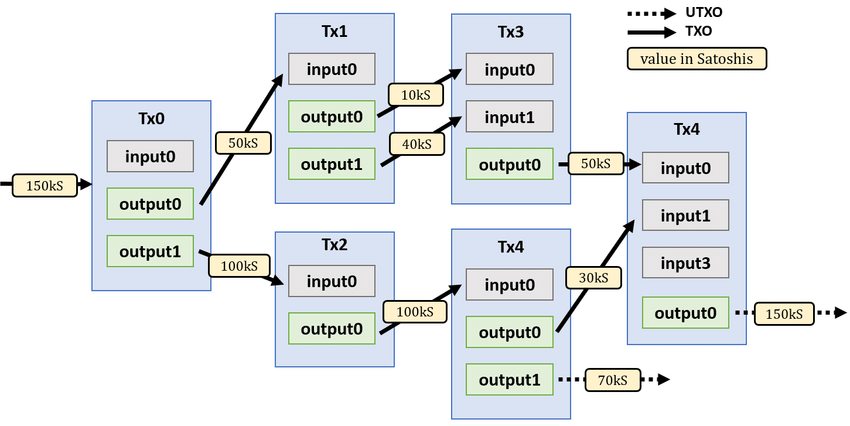
\includegraphics[width=\textwidth,clip=false]{pictures/bitcoin-dag.png}
  \end{center}

\end{frame}

\begin{frame}\frametitle{How Alice's wallet prepares a transaction}

  \begin{enumerate}
  \item Alice's wallet keeps a list of all known unspent outputs for the address
    of Alice
    \begin{itemize}
    \item if it does not know it, it can query the bitcoin network through an API
    \end{itemize}
  \item the wallet selects a subset $\mathit{inputs}$ of the unspent outputs, enough to cover
    the $\mathit{amount}$ of the transaction and signs to prove she's their owner
    \begin{itemize}
    \item any strategy can be applied here
    \end{itemize}
  \item the wallet specifies an output for the destination address of the transaction
    and the $\mathit{amount}\ge 0$ sent to that output
  \item the wallet specifies a second output, normally Alice's address itself, and the
    $\mathit{change}\ge 0$ sent back to Alice
  \item the difference
    \[
    \mathit{fee}=\sum\mathit{inputs}-\mathit{amount}-\mathit{change}\ge 0
    \]
    is the network's reward (and protection) for processing the transaction
  \end{enumerate}

\end{frame}

\begin{frame}\frametitle{How Alice sends the transaction}

  \begin{enumerate}
  \item Alice's wallet sends the bytes of the transaction to a node of the
    bitcoin p2p network
  \item the transaction gets forwarded among all peers (flooding)
  \item the wallet of the destination will very soon see a transaction
    for its address and can assume that it will eventually be processed
    (\alert{unconfirmed transaction})
  \item eventually, around $10$ minutes later,
    the transaction will be processed by the network and
    the wallet of the destination will notice that (\alert{confirmed transaction})
  \item after some time, around one hour, the transaction can be considered
    as definitively processed (\alert{finalized transaction})
  \end{enumerate}

  Merchants can wait for 3, 4 or 5 before handling over the good,
  depending on the relevance of the transaction

\end{frame}

\begin{frame}\frametitle{Miners and Rewards}

  \begin{greenbox}{Miners are (some) nodes of the bitcoin network. They receive, forward
      and aggregate transactions into collectors, called \alert{blocks}}
    When a node creates a new block, it has the right to tag the block
    with a bitcoin address $\mu$, called the \alert{miner}'s address:
    \begin{itemize}
    \item the fees $\phi_1\cdots\phi_n$ of the $n$ transactions in the block go to $\mu$
    \item some amount of money $\iota$ is created out of thin air and goes to $\mu$
    \end{itemize}
  \end{greenbox}

  \bigskip

  \begin{greenbox}{}
    Typically, $\mu$ belongs to the person/organization who owns the machine that runs the node
  \end{greenbox}

  \bigskip

  \begin{greenbox}{}
    $\iota$ is the \alert{inflation}: it is computed through a fixed algorithm that makes it decrease with the time
    and will eventually reach $0$, the day when 21,000,000 total bitcoins will be mined
    \begin{itemize}
    \item[$\Rightarrow$] bitcoin is deflationary
    \end{itemize}
  \end{greenbox}

\end{frame}

\begin{frame}\frametitle{Bitcoin supply over the years}

  \begin{center}
    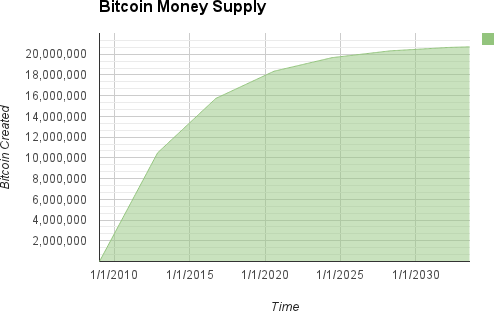
\includegraphics[width=\textwidth,clip=false]{pictures/mbc2_1001.png}
  \end{center}

\end{frame}

\begin{frame}\frametitle{How miners work}

  \begin{enumerate}
    \item Each miner listens the p2p network for new transactions and stores them in a
      temporary area called mempool
    \item when enough new transactions are available in the mempool, it selects some of them
      \begin{itemize}
      \item typically, it selects those with the largest fees, but any other choice is fine: different miners can use different strategies
      \end{itemize}
    \item it builds a new block (\alert{mining}):
      \begin{itemize}
      \item it adds the selected transactions
      \item it adds a special \alert{coinbase transaction} with no inputs, whose only output is $\mu$
        and whose amount is $\iota+\sum_{i=1}^n\phi_i$
      \item it tags the block with a reference to the previous block
      \item if no other miner has been faster, it forwards the new block to all its peers
      \end{itemize}
  \end{enumerate}
\end{frame}

\begin{frame}\frametitle{Block's height, depth and confirmations}

  \begin{center}
    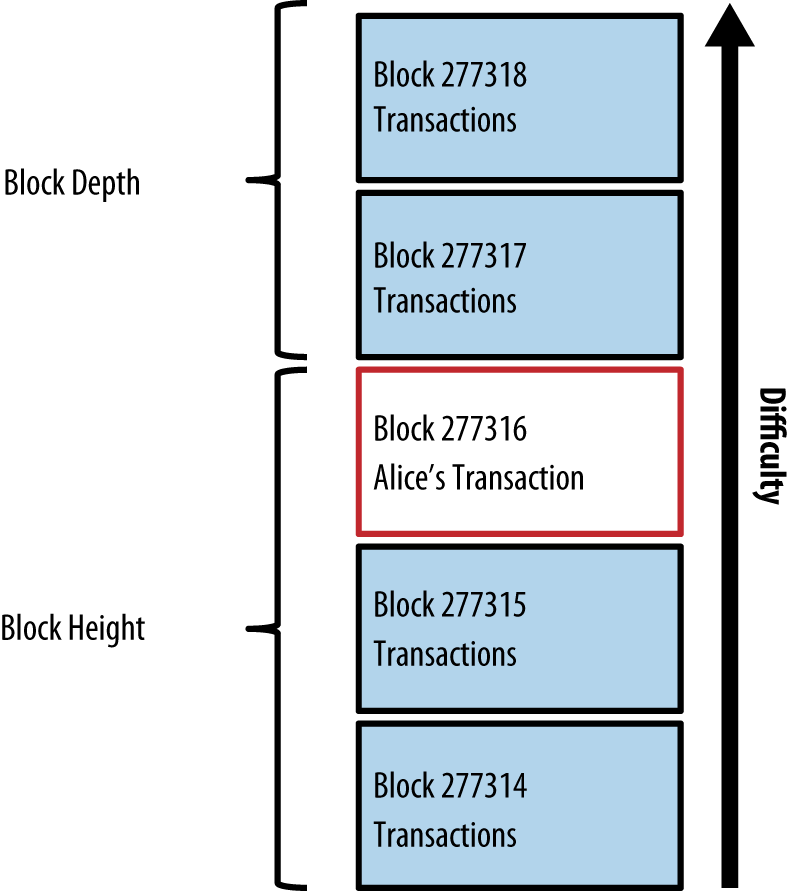
\includegraphics[scale=1,clip=false]{pictures/mbc2_0209.png}
  \end{center}

\end{frame}

\begin{frame}[fragile]\frametitle{The transaction}

  \begin{center}
    no coins, no senders, no recipients, no balances, no accounts, no addresses
  \end{center}

  {\scriptsize\begin{alltt}
\{
  "vins": [
    \{
      "txid": "7957a35fe64f80d234d76d83a2a8f1a0d8149a41d81de548f0a65a8a999f6f18",
      "vout": 0,
      "unlock": "3045022100884d142d86652a3f47... 0484ecc0d46f..."
    \}
  ],
  "vouts": [
    \{
      "value": 0.01500000,
      "lock": "DUP HASH160 ab68025513c3dbd2f7b92a94e0581f5d50f654e7 
               EQUALVERIFY CHECKSIG"
    \},
    \{
      "value": 0.08450000,
      "lock": "DUP HASH160 7f9b1a7fb68d60c536c2fd8aeaa53a8f3cc025a8
               EQUALVERIFY CHECKSIG"
    \}
  ]
\}
\end{alltt}}

\end{frame}

\begin{frame}[fragile]\frametitle{The real transaction}

  \begin{center}
    two new UTXOs (unspent transaction outputs)
  \end{center}

  {\scriptsize\begin{alltt}
\{
  "vins": [
    \{
      "txid": "7957a35fe64f80d234d76d83a2a8f1a0d8149a41d81de548f0a65a8a999f6f18",
      "vout": 0,
      "unlock": "3045022100884d142d86652a3f47... 0484ecc0d46f..."
    \}
  ],
  \color{red}{"vouts": [
    \{
      "value": 0.01500000,
      "lock": "DUP HASH160 ab68025513c3dbd2f7b92a94e0581f5d50f654e7
               EQUALVERIFY CHECKSIG"
    \},
    \{
      "value": 0.08450000,
      "lock": "DUP HASH160 7f9b1a7fb68d60c536c2fd8aeaa53a8f3cc025a8
               EQUALVERIFY CHECKSIG",
    \}
  ]}
\}
\end{alltt}}

\end{frame}

\begin{frame}[fragile]\frametitle{The real transaction}

  \begin{center}
    reference to an old UTXO (soon to be TXO)
  \end{center}

  {\scriptsize\begin{alltt}
\{
  \alert{"vins": [
    \{
      "txid": "7957a35fe64f80d234d76d83a2a8f1a0d8149a41d81de548f0a65a8a999f6f18",
      "vout": 0,
      "unlock": "3045022100884d142d86652a3f47... 0484ecc0d46f..."
    \}
  ]},
  "vouts": [
    \{
      "value": 0.01500000,
      "lock": "DUP HASH160 ab68025513c3dbd2f7b92a94e0581f5d50f654e7
               EQUALVERIFY CHECKSIG"
    \},
    \{
      "value": 0.08450000,
      "lock": "DUP HASH160 7f9b1a7fb68d60c536c2fd8aeaa53a8f3cc025a8
               EQUALVERIFY CHECKSIG"
    \}
  ]
\}
\end{alltt}}

\end{frame}

\begin{frame}[fragile]\frametitle{The real transaction}

  \begin{center}
    the amount of the first new UTXO (in satoshis)
  \end{center}

  {\scriptsize\begin{alltt}
\{
  "vins": [
    \{
      "txid": "7957a35fe64f80d234d76d83a2a8f1a0d8149a41d81de548f0a65a8a999f6f18",
      "vout": 0,
      "unlock": "3045022100884d142d86652a3f47... 0484ecc0d46f..."
    \}
  ],
  "vouts": [
    \{
      \alert{"value": 0.01500000},
      "lock": "DUP HASH160 ab68025513c3dbd2f7b92a94e0581f5d50f654e7
               EQUALVERIFY CHECKSIG"
    \},
    \{
      "value": 0.08450000,
      "lock": "DUP HASH160 7f9b1a7fb68d60c536c2fd8aeaa53a8f3cc025a8
               EQUALVERIFY CHECKSIG"
    \}
  ]
\}
\end{alltt}}

\end{frame}

\begin{frame}[fragile]\frametitle{The real transaction}

  \begin{center}
    the unlocking or witness script of the first new UTXO (crypto-puzzle)
  \end{center}

  {\scriptsize\begin{alltt}
\{
  "vins": [
    \{
      "txid": "7957a35fe64f80d234d76d83a2a8f1a0d8149a41d81de548f0a65a8a999f6f18",
      "vout": 0,
      "unlock": "3045022100884d142d86652a3f47... 0484ecc0d46f..."
    \}
  ],
  "vouts": [
    \{
      "value": 0.01500000,
      \alert{"lock": "DUP HASH160 ab68025513c3dbd2f7b92a94e0581f5d50f654e7
               EQUALVERIFY CHECKSIG"}
    \},
    \{
      "value": 0.08450000,
      "lock": "DUP HASH160 7f9b1a7fb68d60c536c2fd8aeaa53a8f3cc025a8
               EQUALVERIFY CHECKSIG"
    \}
  ]
\}
\end{alltt}}

\end{frame}

\begin{frame}[fragile]\frametitle{The real transaction}

  \begin{center}
    the hash of the transaction whose $\mathtt{vout}^{\mathit{th}}$ UTXO is being spent
  \end{center}

  {\scriptsize\begin{alltt}
\{
  "vins": [
    \{
      \alert{"txid": "7957a35fe64f80d234d76d83a2a8f1a0d8149a41d81de548f0a65a8a999f6f18",
      "vout": 0},
      "unlock": "3045022100884d142d86652a3f47... 0484ecc0d46f..."
    \}
  ],
  "vouts": [
    \{
      "value": 0.01500000,
      "lock": "DUP HASH160 ab68025513c3dbd2f7b92a94e0581f5d50f654e7
               EQUALVERIFY CHECKSIG"
    \},
    \{
      "value": 0.08450000,
      "lock": "DUP HASH160 7f9b1a7fb68d60c536c2fd8aeaa53a8f3cc025a8
               EQUALVERIFY CHECKSIG"
    \}
  ]
\}
\end{alltt}}

\end{frame}

\begin{frame}[fragile]\frametitle{The real transaction}

  \begin{center}
    the unlocking script (usually digital signature + public key)
  \end{center}

  {\scriptsize\begin{alltt}
\{
  "vins": [
    \{
      "txid": "7957a35fe64f80d234d76d83a2a8f1a0d8149a41d81de548f0a65a8a999f6f18",
      "vout": 0,
      \alert{"unlock": "3045022100884d142d86652a3f47... 0484ecc0d46f..."}
    \}
  ],
  "vouts": [
    \{
      "value": 0.01500000,
      "lock": "DUP HASH160 ab68025513c3dbd2f7b92a94e0581f5d50f654e7
               EQUALVERIFY CHECKSIG"
    \},
    \{
      "value": 0.08450000,
      "lock": "DUP HASH160 7f9b1a7fb68d60c536c2fd8aeaa53a8f3cc025a8
               EQUALVERIFY CHECKSIG",
    \}
  ]
\}
\end{alltt}}

\end{frame}

\begin{frame}[fragile]\frametitle{The real transaction}

  \begin{center}
    scripts are written in the Script programming language
  \end{center}

  {\scriptsize\begin{alltt}
\{
  "vins": [
    \{
      "txid": "7957a35fe64f80d234d76d83a2a8f1a0d8149a41d81de548f0a65a8a999f6f18",
      "vout": 0,
      "unlock": \alert{"3045022100884d142d86652a3f47... 0484ecc0d46f..."}
    \}
  ],
  "vouts": [
    \{
      "value": 0.01500000,
      "lock": \alert{"DUP HASH160 ab68025513c3dbd2f7b92a94e0581f5d50f654e7
               EQUALVERIFY CHECKSIG"}
    \},
    \{
      "value": 0.08450000,
      "lock": \alert{"DUP HASH160 7f9b1a7fb68d60c536c2fd8aeaa53a8f3cc025a8
               EQUALVERIFY CHECKSIG"}
    \}
  ]
\}
\end{alltt}}

\end{frame}

\begin{frame}\frametitle{The Script programming language}

  \begin{greenbox}{Reverse-polish stack-based stateless language}
    \begin{itemize}
    \item[{
\includegraphics[scale=0.03]{pictures/check.png}}] sequence
    \item[{
\includegraphics[scale=0.03]{pictures/check.png}}] conditional
    \item[{
\includegraphics[scale=0.0135]{pictures/uncheck.png}}] repetition
    \end{itemize}

    \begin{center}
      \alert{$\Rightarrow$ Turing incomplete}
    \end{center}

  \end{greenbox}

  \bigskip

  \begin{greenbox}{Why Turing incomplete?}
    \begin{enumerate}
    \item predictable execution time
    \item guaranteed termination
    \end{enumerate}

    \begin{center}
      denial of service attacks are impossible \emph{at language level}
    \end{center}

  \end{greenbox}

\end{frame}

\begin{frame}\frametitle{Script validity}

  \begin{greenbox}{}
    A program in the Script language is \alert{valid} if its execution
    does not stop with failure and terminates with a stack whose topmost element is \texttt{TRUE}
  \end{greenbox}

  \bigskip

  \begin{greenbox}{Execution proceeds left-to-right}
    Let us execute \texttt{2 3 ADD 5 EQUAL} to see if it's valid
  \end{greenbox}

\end{frame}

\begin{frame}\frametitle{\texttt{2 3 ADD 5 EQUAL}}

  \begin{center}
    \only<1>{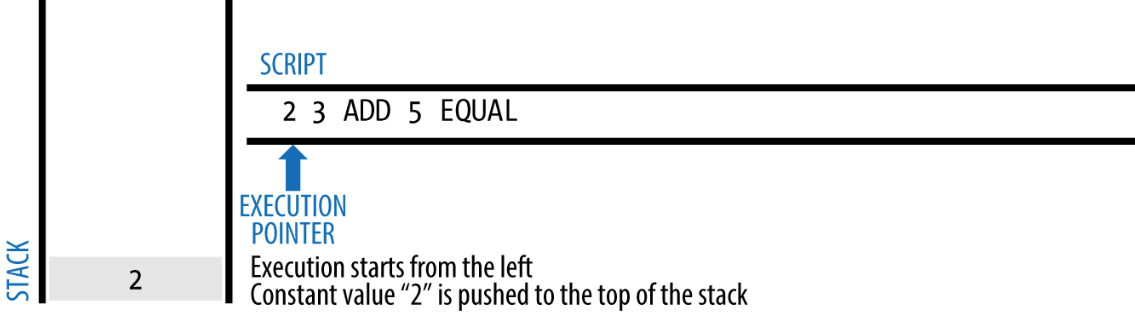
\includegraphics[width=\textwidth,clip=false]{pictures/stack1.png}}
    \only<2>{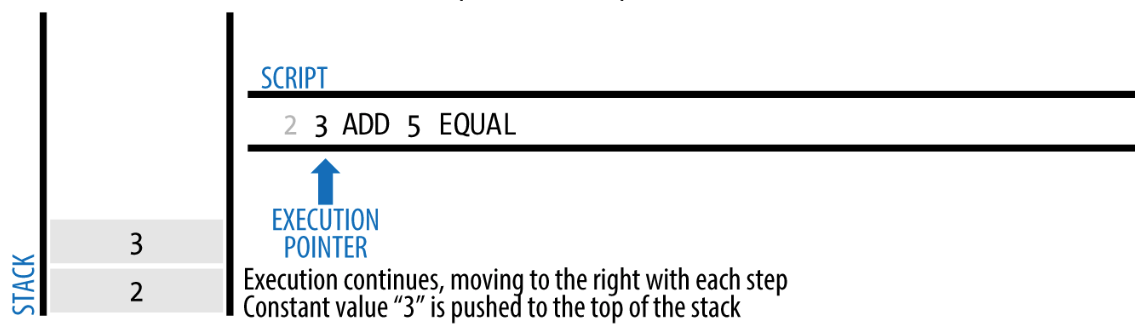
\includegraphics[width=\textwidth,clip=false]{pictures/stack2.png}}
    \only<3>{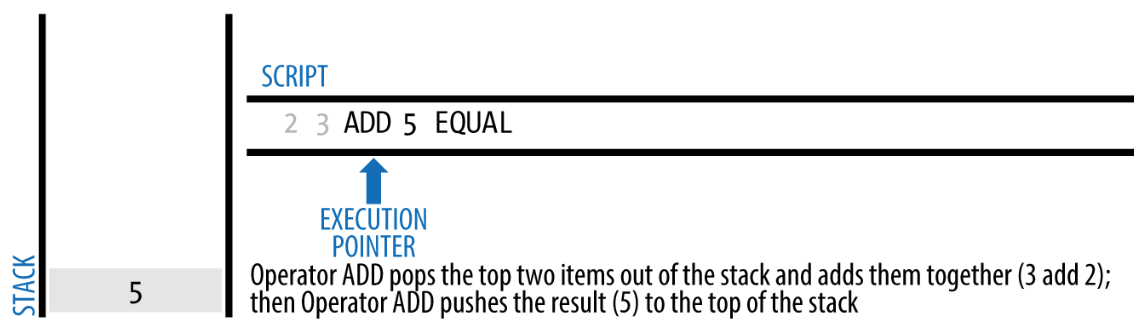
\includegraphics[width=\textwidth,clip=false]{pictures/stack3.png}}
    \only<4>{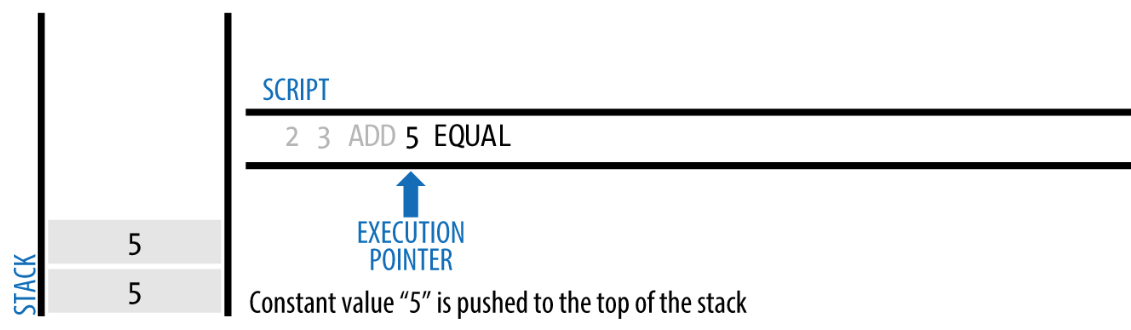
\includegraphics[width=\textwidth,clip=false]{pictures/stack4.png}}
    \only<5>{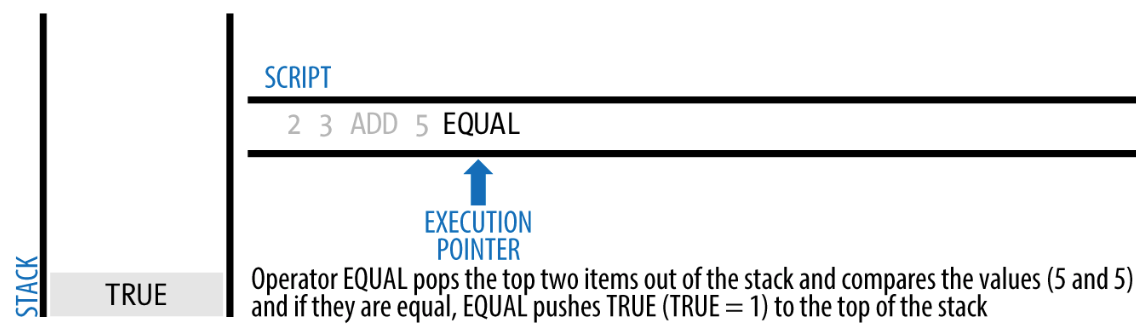
\includegraphics[width=\textwidth,clip=false]{pictures/stack5.png}}
  \end{center}

  \begin{center}
    \only<5>{The program is valid!}
  \end{center}

\end{frame}

\begin{frame}\frametitle{Other examples of (in-)valid scripts}

  \begin{greenbox}{These are all valid}
    \begin{itemize}
    \item \texttt{TRUE}
    \item \texttt{FALSE TRUE}
    \item \texttt{2 7 ADD 3 SUB 1 ADD 7 EQUAL}
    \item \texttt{2 7 EQUAL IF FALSE ELSE TRUE ENDIF}
    \end{itemize}
  \end{greenbox}

  \bigskip

  \begin{greenbox}{These are all invalid}
    \begin{itemize}
    \item \texttt{FALSE}
    \item \texttt{2 7 EQUAL}
    \item \texttt{2 7 EQUAL IF TRUE ELSE FALSE ENDIF}
    \item \texttt{2 7 EQUAL TRUE ENDIF}
    \end{itemize}
  \end{greenbox}

\end{frame}

\begin{frame}[fragile]\frametitle{The validation algorithm for bitcoin transactions}

{\scriptsize\begin{alltt}
previous_tx = \{ // this transaction has hash H
  "vins": .....
  "vouts": [ \{ "value": .....,     "lock": "....." \}, ..... ]
\}

tx = \{
  "vins": [ \{ "txid": H,     "vout": .....,     "unlock": "....." \}, ..... ],
  "vouts": .....
\}
\end{alltt}}

    {\small\begin{alltt}
    boolean is_valid(Transaction tx) \{
      for each (txid, vout, unlock) in tx.vins
        previous_tx = \alert{get_transaction}(txid)
        lock = previous_tx.vouts[vout].lock
        if ({\color{blue}{unlock lock}} is invalid)
          return false

      return true
    \}
    \end{alltt}}

\end{frame}

\begin{frame}[fragile]\frametitle{The typical P2PKH script (\emph{pay to publickey hash})}

\begin{greenbox}{``I want to send some value to \<address>''}
{\scriptsize\begin{alltt}
previous_tx = \{ // this transaction has hash H
  "vins": .....
  "vouts": [\{ "value": ..., "lock": {\color{blue}{DUP HASH160 <address> EQUALVERIFY CHECKSIG}} \},
            .....]
\}
\end{alltt}}
\end{greenbox}

\bigskip

\begin{greenbox}{``I'm \<address>, here is my signature, use that value''}
{\scriptsize\begin{alltt}
tx = \{
  "vins": [ \{ "txid": H,   "vout": .....,   "unlock": {\color{blue}{<sig> <PubK>}}\}, ..... ],
  "vouts": .....
\}
\end{alltt}}
\end{greenbox}

\bigskip

\begin{greenbox}{\<unlock lock>}
  \begin{center}
    \texttt{<sig> <PubK> DUP HASH160 <address> EQUALVERIFY CHECKSIG}
  \end{center}
\end{greenbox}

The bitcoin \<address> is often referred to as \<PublicKHash>

\end{frame}

\begin{frame}\frametitle{\texttt{<sig> <PubK> DUP HASH160 <address> EQUALVERIFY CHECKSIG}}

  \begin{center}
    \only<1>{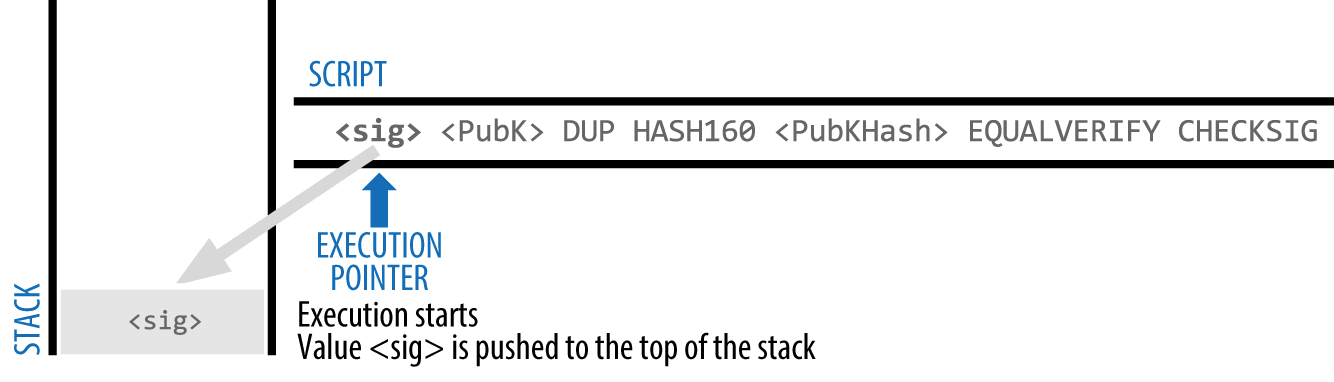
\includegraphics[width=\textwidth,clip=false]{pictures/p2pkh1.png}}
    \only<2>{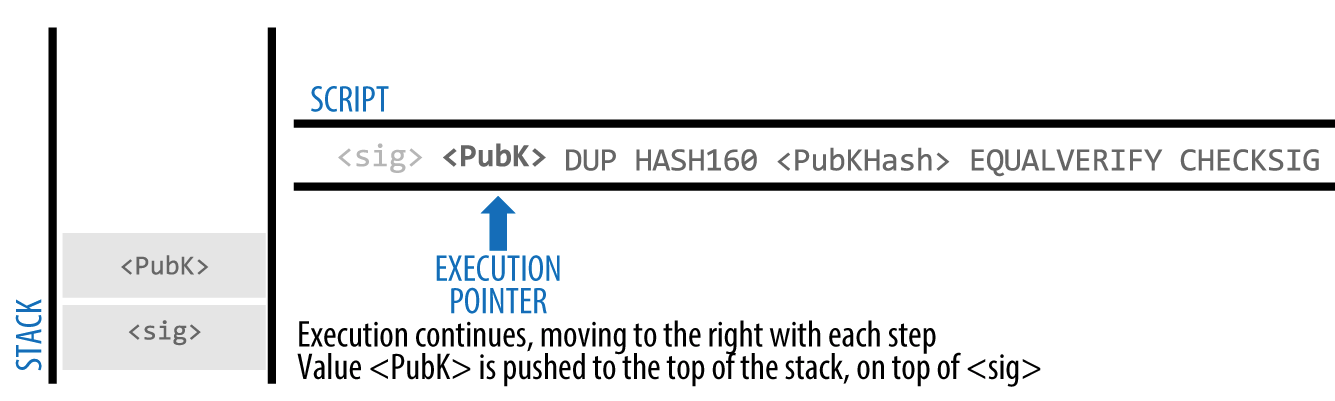
\includegraphics[width=\textwidth,clip=false]{pictures/p2pkh2.png}}
    \only<3>{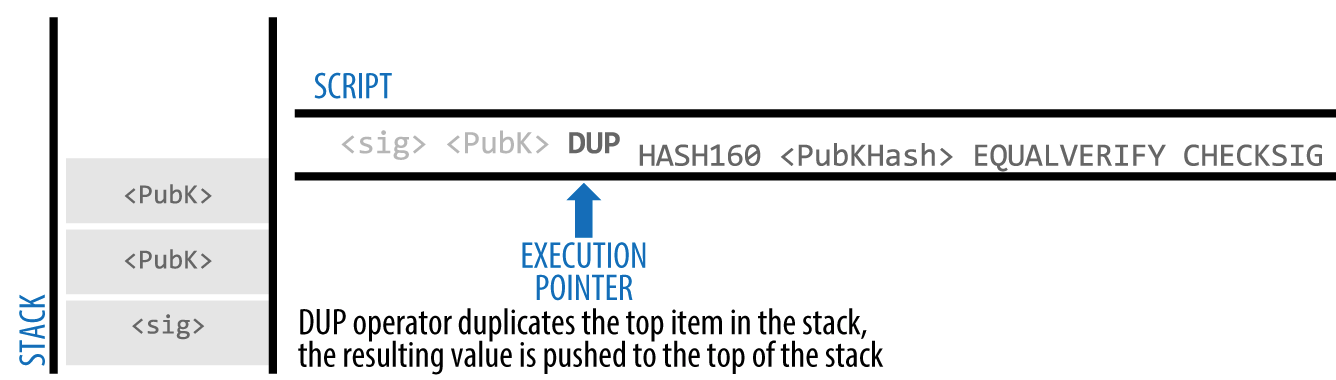
\includegraphics[width=\textwidth,clip=false]{pictures/p2pkh3.png}}
    \only<4>{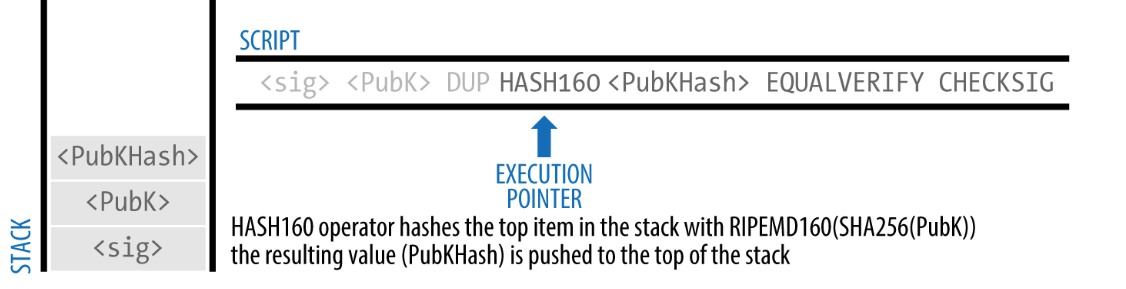
\includegraphics[width=\textwidth,clip=false]{pictures/p2pkh4.png}}
    \only<5>{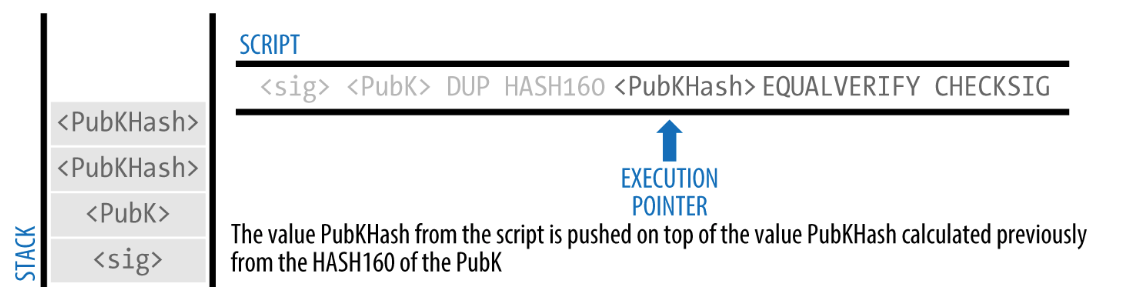
\includegraphics[width=\textwidth,clip=false]{pictures/p2pkh5.png}}
    \only<6-7>{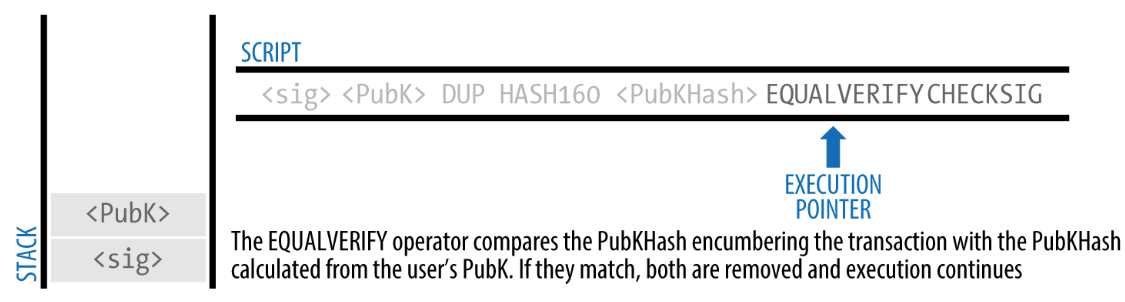
\includegraphics[width=\textwidth,clip=false]{pictures/p2pkh6.png}}+
    \only<8>{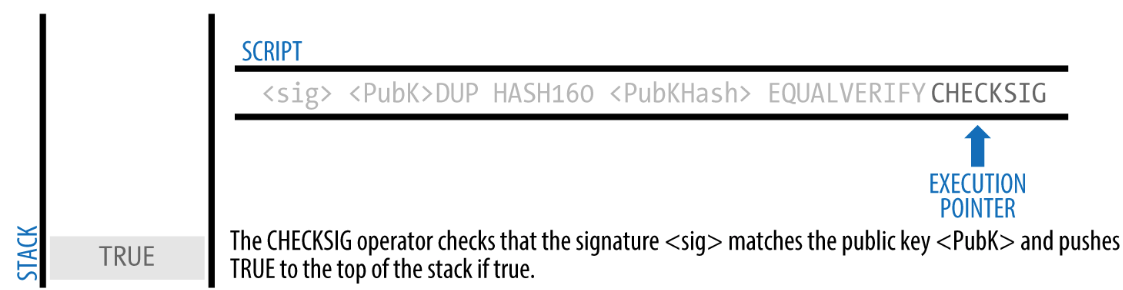
\includegraphics[width=\textwidth,clip=false]{pictures/p2pkh7.png}}
  \end{center}

  \uncover<7>{
    \begin{greenbox}{}
      \<CHECKSIG> verifies that \<sig> is a signature of the transaction
      generated by using the private key corresponsing to \<pubK>
    \end{greenbox}
  }

  \uncover<8>{
    \begin{center}
      This script gives proof of ownership!
    \end{center}
  }

\end{frame}

\begin{frame}\frametitle{Properties of Bitcoin's transactions}

  \begin{itemize}
  \item Script programs are only used to check the validity of the transactions
  \item Script programs never modify the state of the system
  \item Transactions undo is very easy (they just move money around)
  \end{itemize}

\end{frame}

\begin{frame}\frametitle{Block headers contain the hash of all transactions in the block (Merkle root)}

  \begin{center}
    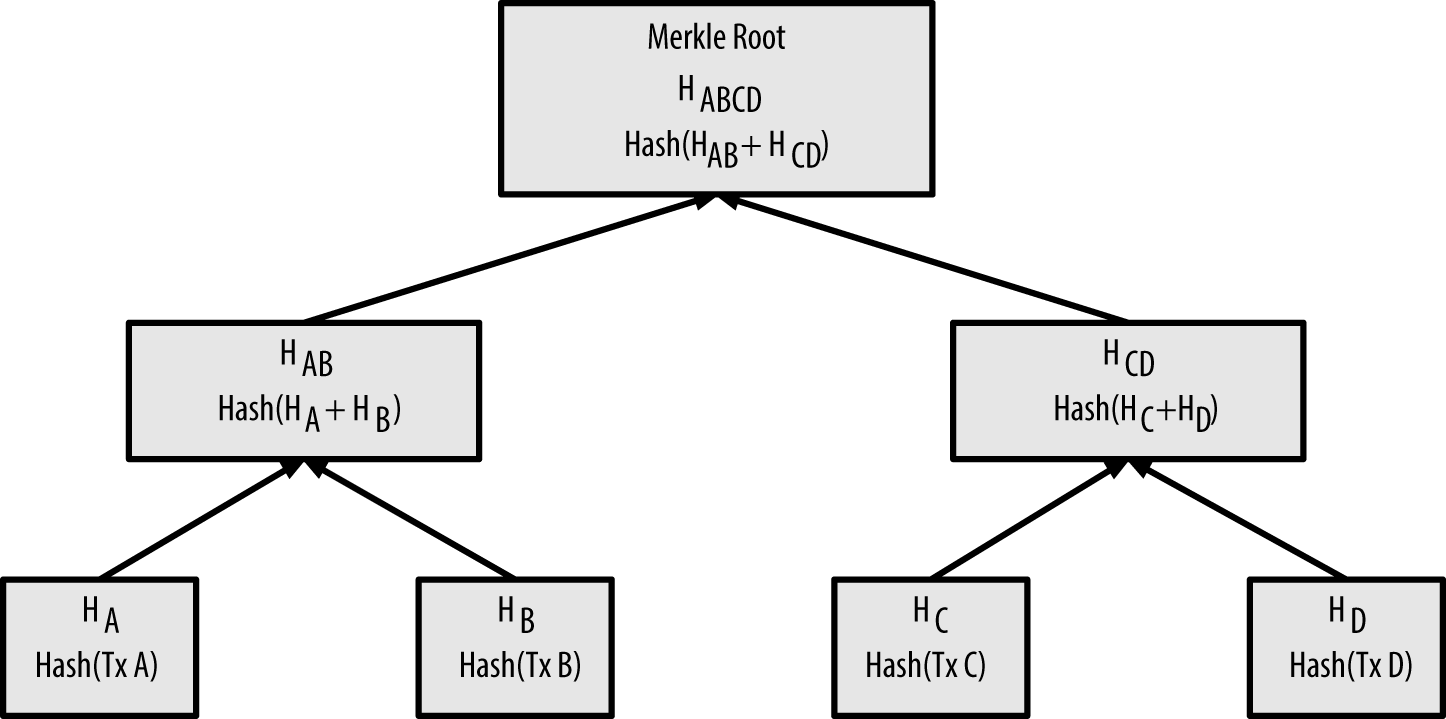
\includegraphics[width=\textwidth,clip=false]{pictures/mbc2_0902.png}
  \end{center}

\end{frame}

\begin{frame}\frametitle{Merkle trees provide an efficient inclusion test}

  \begin{center}
    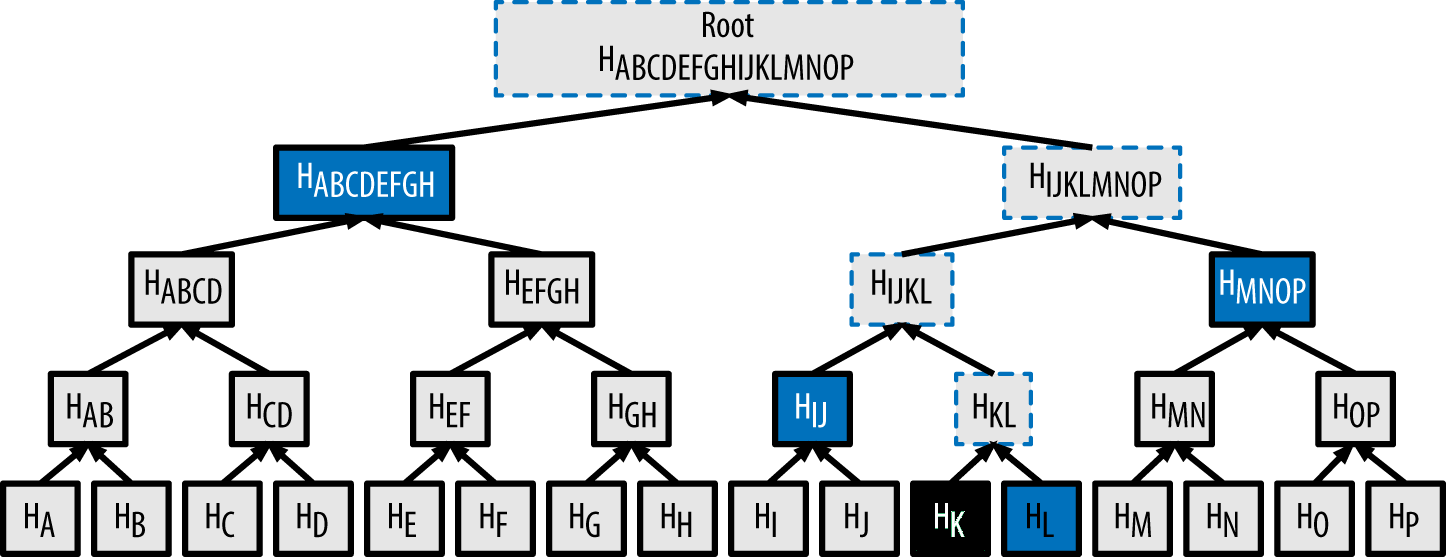
\includegraphics[width=\textwidth,clip=false]{pictures/mbc2_0905.png}
  \end{center}

  \begin{greenbox}{I know the root hash and want to know if the {\color{black}black $H_K$} is included}
    The {\color{blue}four blue hashes} can be given to me as that proof of inclusion
    (\emph{authentication path})
  \end{greenbox}

\end{frame}

\section{Proof of work}

\begin{frame}\frametitle{Mining}

  \begin{center}
    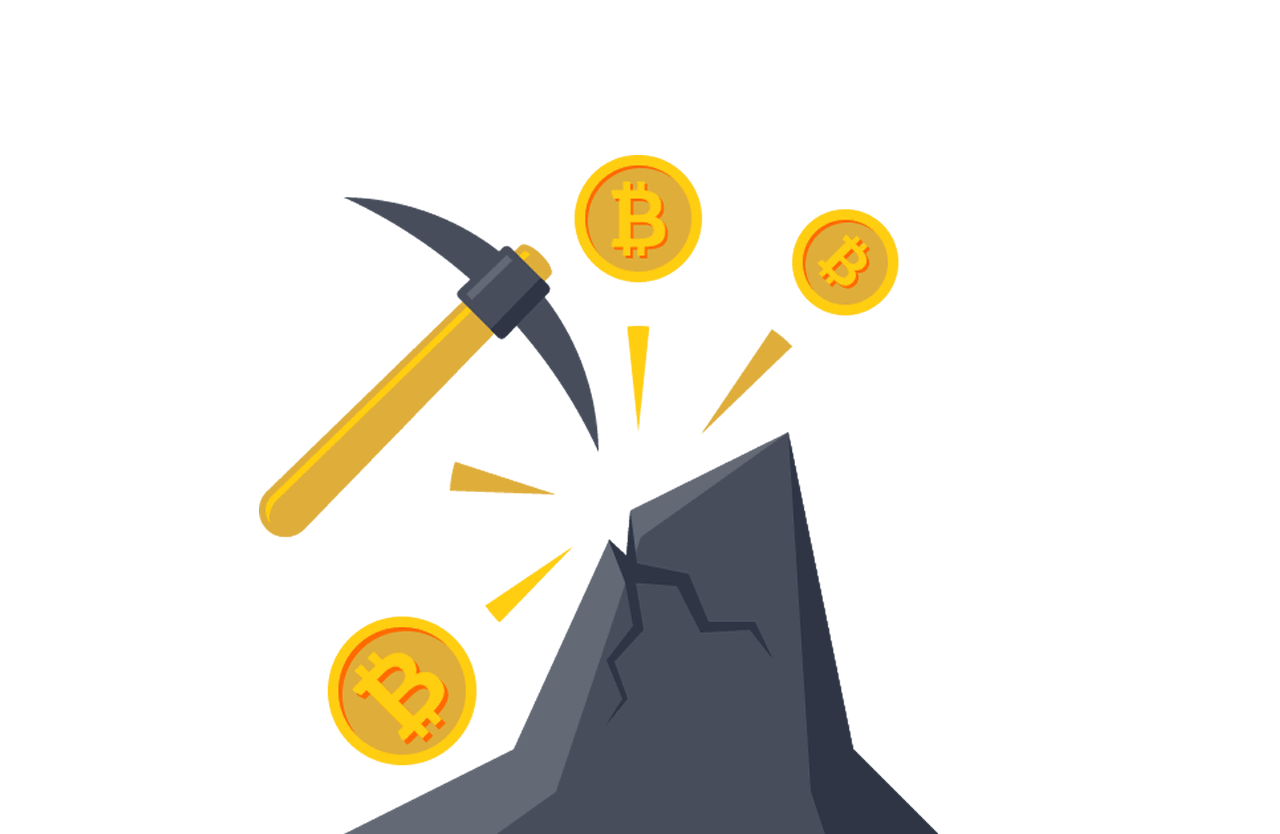
\includegraphics[scale=0.1,clip=false]{pictures/mining.png}
  \end{center}

  \bigskip

  \begin{greenbox}{The vision of the miner}
    The goal of mining is to mint new coins and earn money
  \end{greenbox}

  \bigskip

  \begin{greenbox}{The vision of Nakamoto}
    The goal of mining is to secure the bitcoin network
  \end{greenbox}

\end{frame}

\begin{frame}\frametitle{Miners can only mine correct blocks}

  \begin{greenbox}{New valid block = it respects the {\color{pink}{consensus rules}}}
    \begin{itemize}
    \item the structure of data in the header and transactions must be correct
    \item transactions have at least one input (but for coinbase transactions)
    \item transactions have at least one output
    \item transactions do not create money (but for coinbase transactions)
    \item coinbase transactions have a correct reward
    \item transactions are all valid (their unlocking scripts match the corresponsing locking scripts)
    \item transaction inputs refer to unspent UTXO only
      (\alert{no double-spending inside the same history})
    \item \ldots
    \end{itemize}
  \end{greenbox}

  \medskip

  \begin{redbox}{}
    \begin{center}
      But what about fairness and progress?
    \end{center}
  \end{redbox}

\end{frame}

\begin{frame}\frametitle{How to kill a dictator}

  \begin{greenbox}{Without proof of work}
    A single node dictates the history of the blockchain
    if it is faster than \emph{each} other node
  \end{greenbox}

  \pause
  \bigskip
  \bigskip

  \begin{greenbox}{With proof of work}
    A single node dictates the history of the blockchain
    if it is faster than \emph{the sum of all} other nodes
  \end{greenbox}

\end{frame}

\begin{frame}\frametitle{Proof of work (PoW)}

  \begin{greenbox}{Add the following consensus rule}
    The hash of valid blocks is smaller than
    a given constant $\mathit{difficulty}$
  \end{greenbox}

  \bigskip

  \begin{greenbox}{Miners must work hard now}
    \begin{enumerate}
    \item build a new block
    \item set the nonce field of its header to a random value
    \item compute the hash $h$ of the header
    \item if $h < \mathit{difficulty}$ stop
    \item otherwise, go back to step 2 and try again
    \end{enumerate}
  \end{greenbox}

  \bigskip

  \begin{itemize}
  \item the header of the resulting block is the PoW
  \item the time to solve this puzzle is inversely proportional to $\mathit{difficulty}$
  \item the algorithm can be easily run in parallel, GPU, ASIC
  \end{itemize}

\end{frame}

\begin{frame}\frametitle{Fork: all nodes start with the same vision}

  \begin{center}
    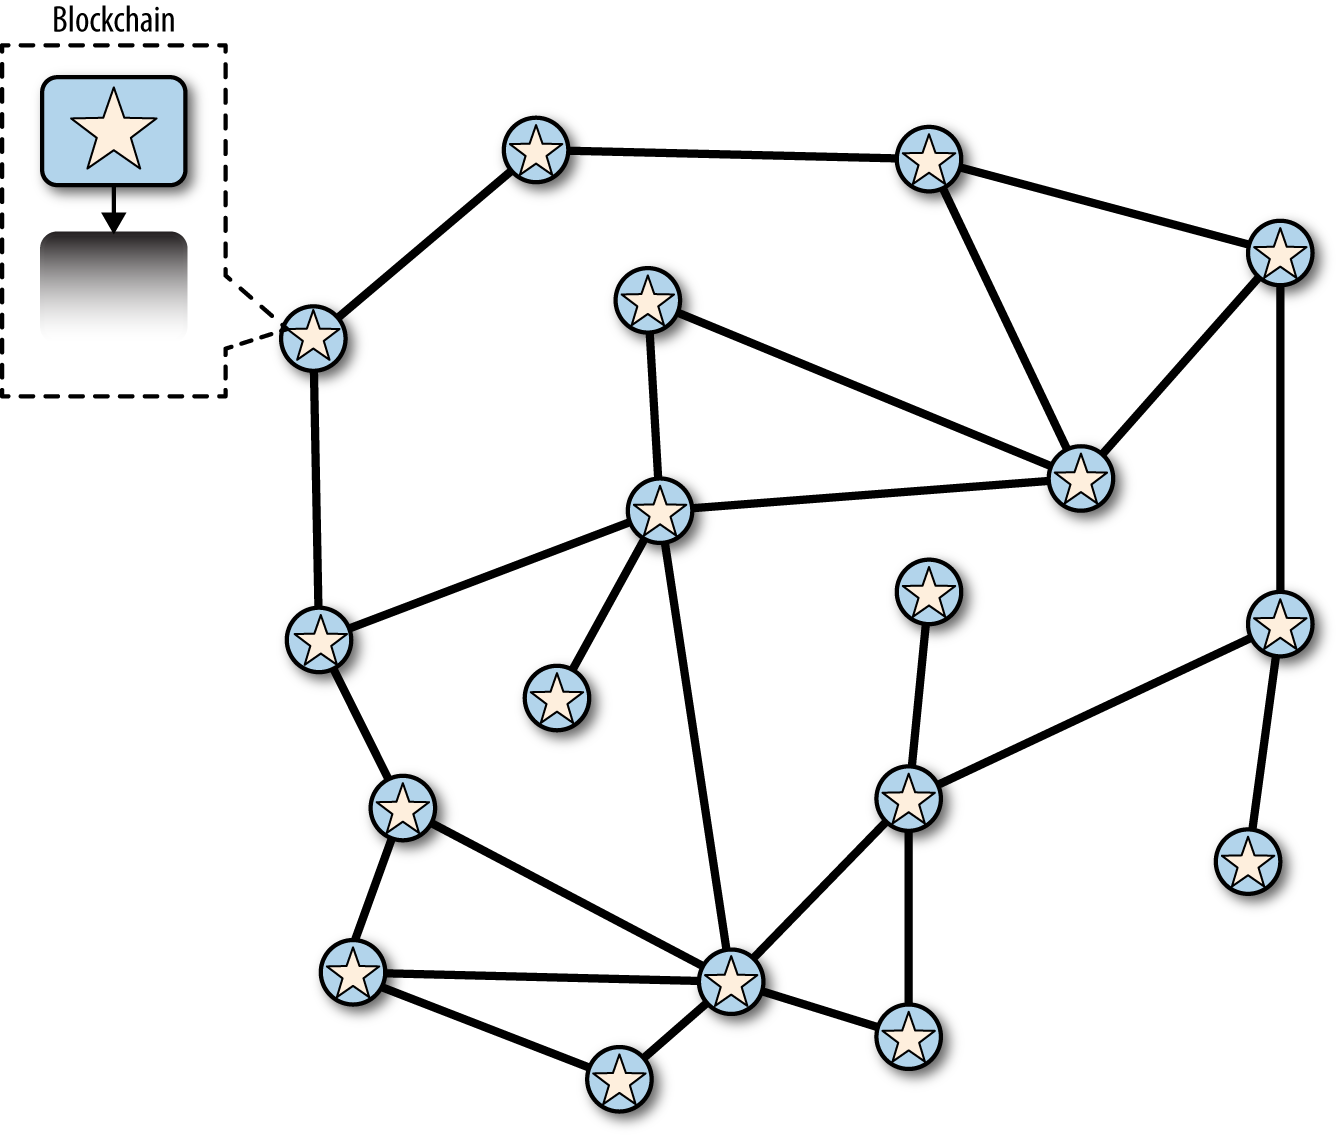
\includegraphics[scale=0.8,clip=false]{pictures/mbc2_1002.png}
  \end{center}

\end{frame}

\begin{frame}\frametitle{Fork: two nodes expand the blockchain simultaneously}

  \begin{center}
    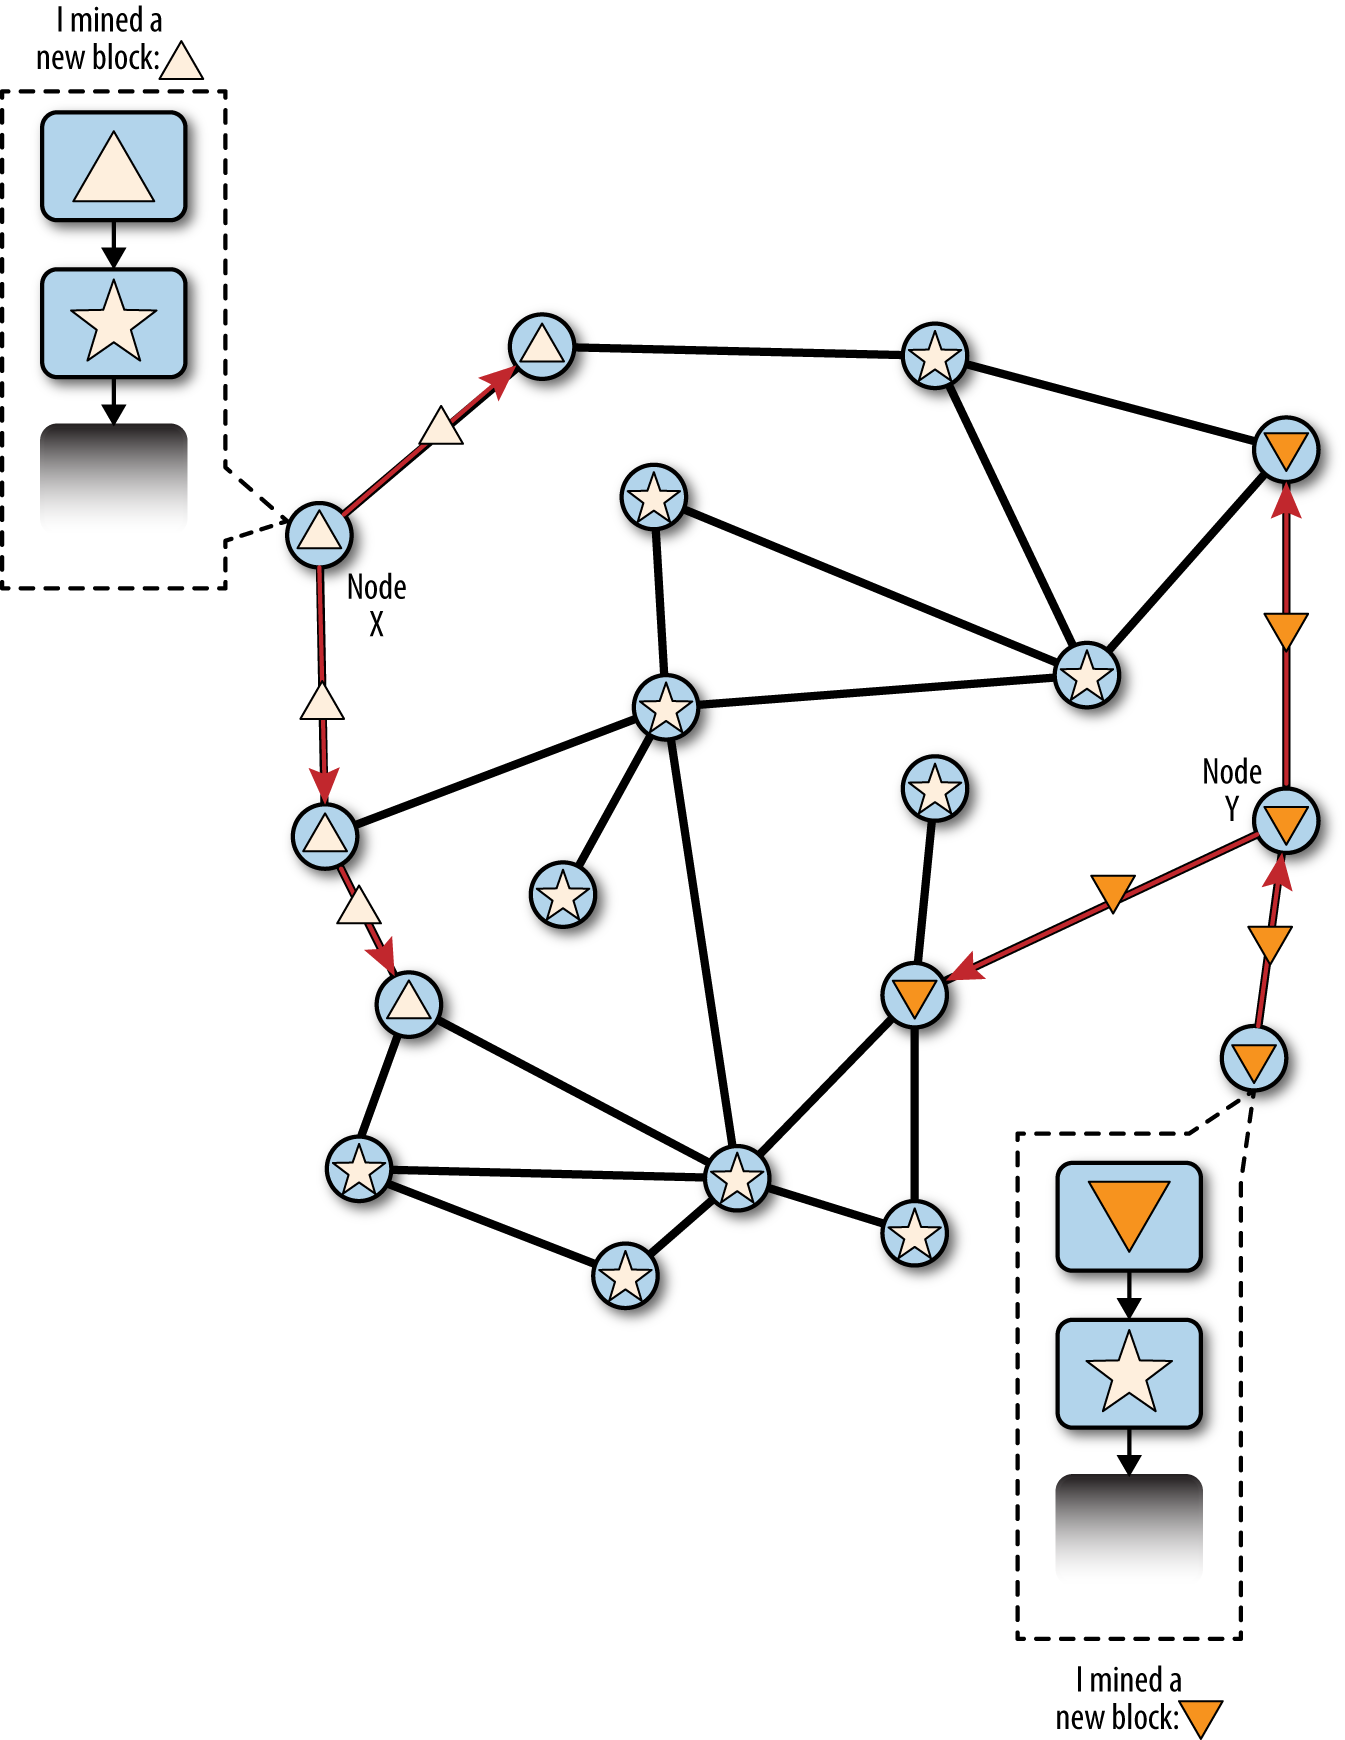
\includegraphics[scale=0.53,clip=false]{pictures/mbc2_1003.png}
  \end{center}

\end{frame}

\begin{frame}\frametitle{Fork: the network is split}

  \begin{center}
    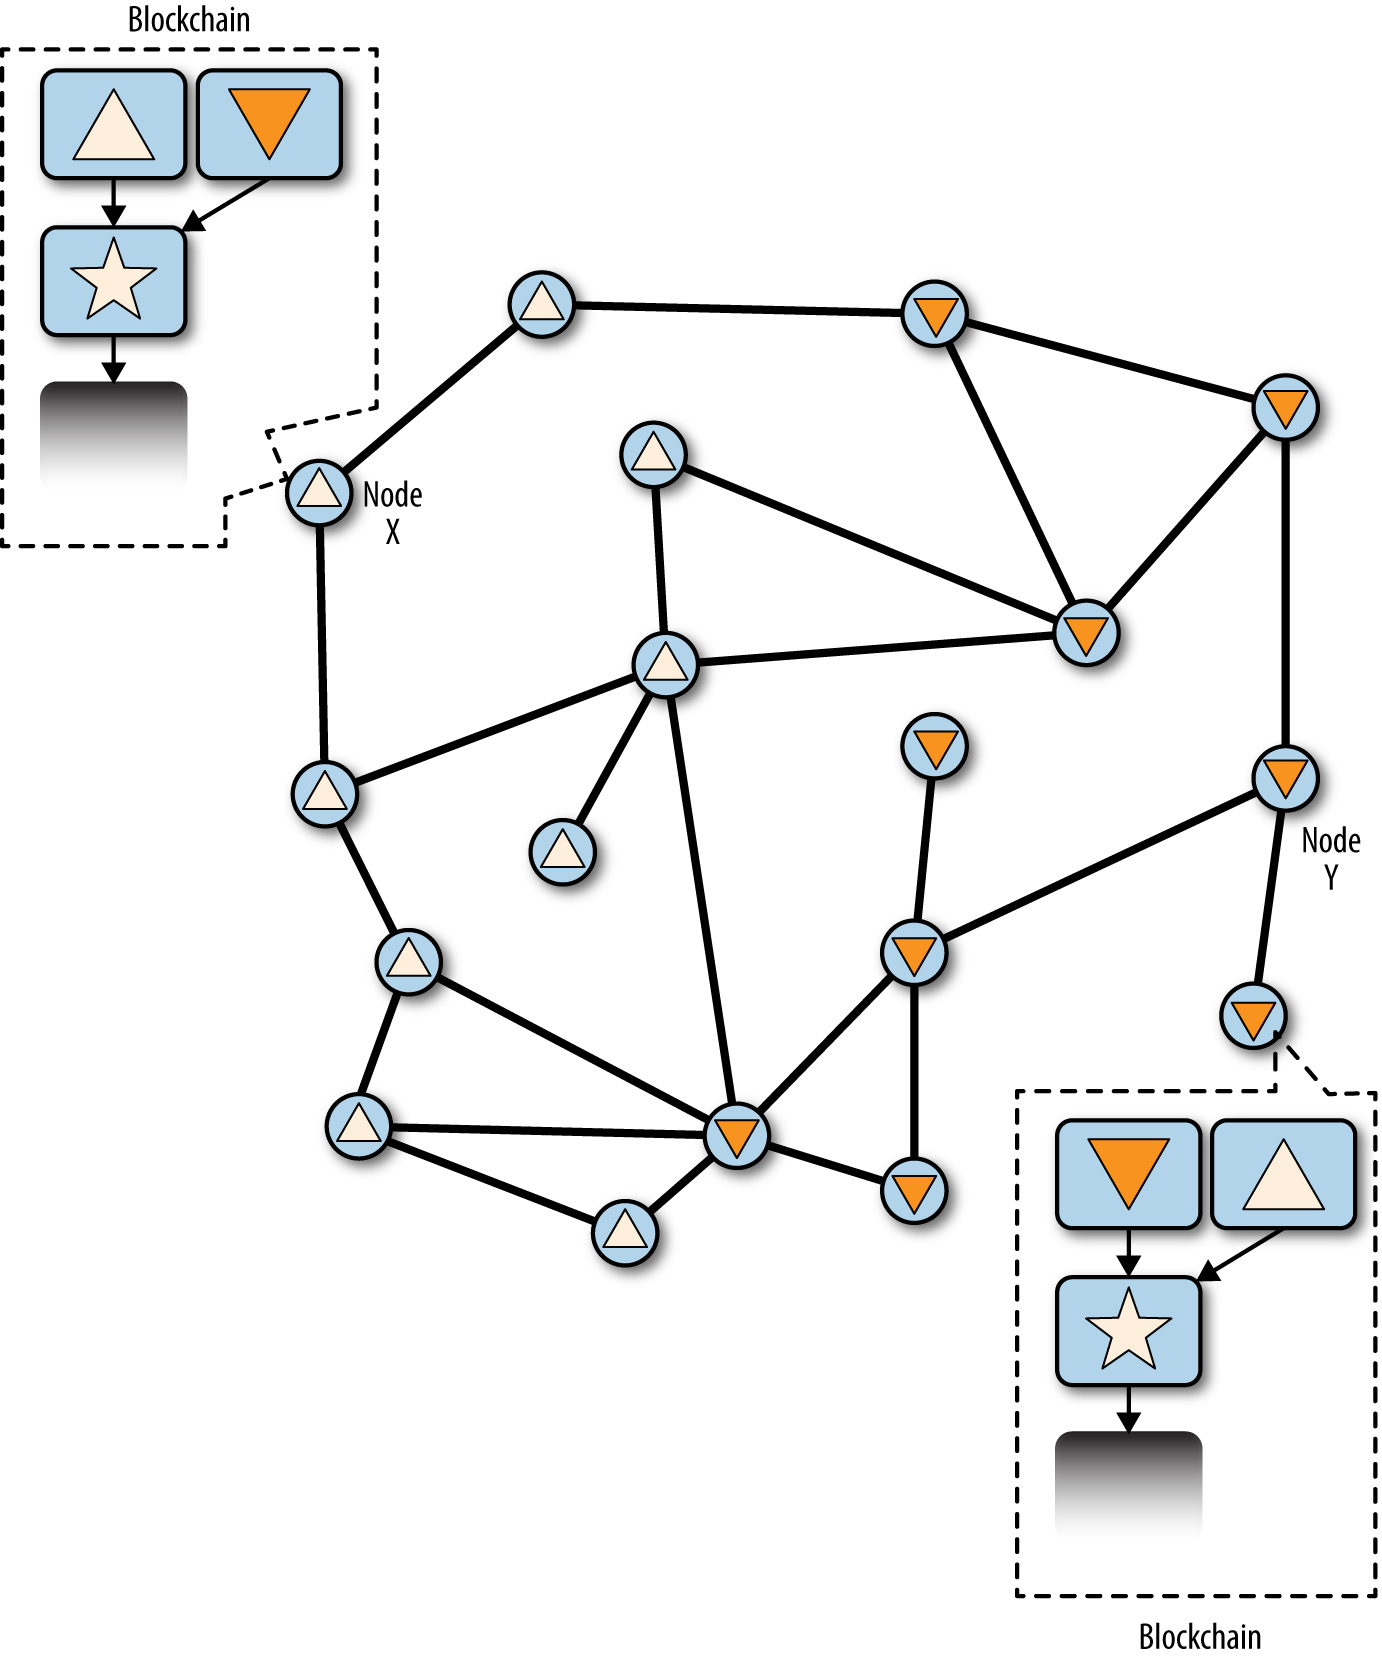
\includegraphics[scale=0.56,clip=false]{pictures/mbc2_1004.png}
  \end{center}

\end{frame}

\begin{frame}\frametitle{Fork: either chain is expanded further}

  \begin{center}
    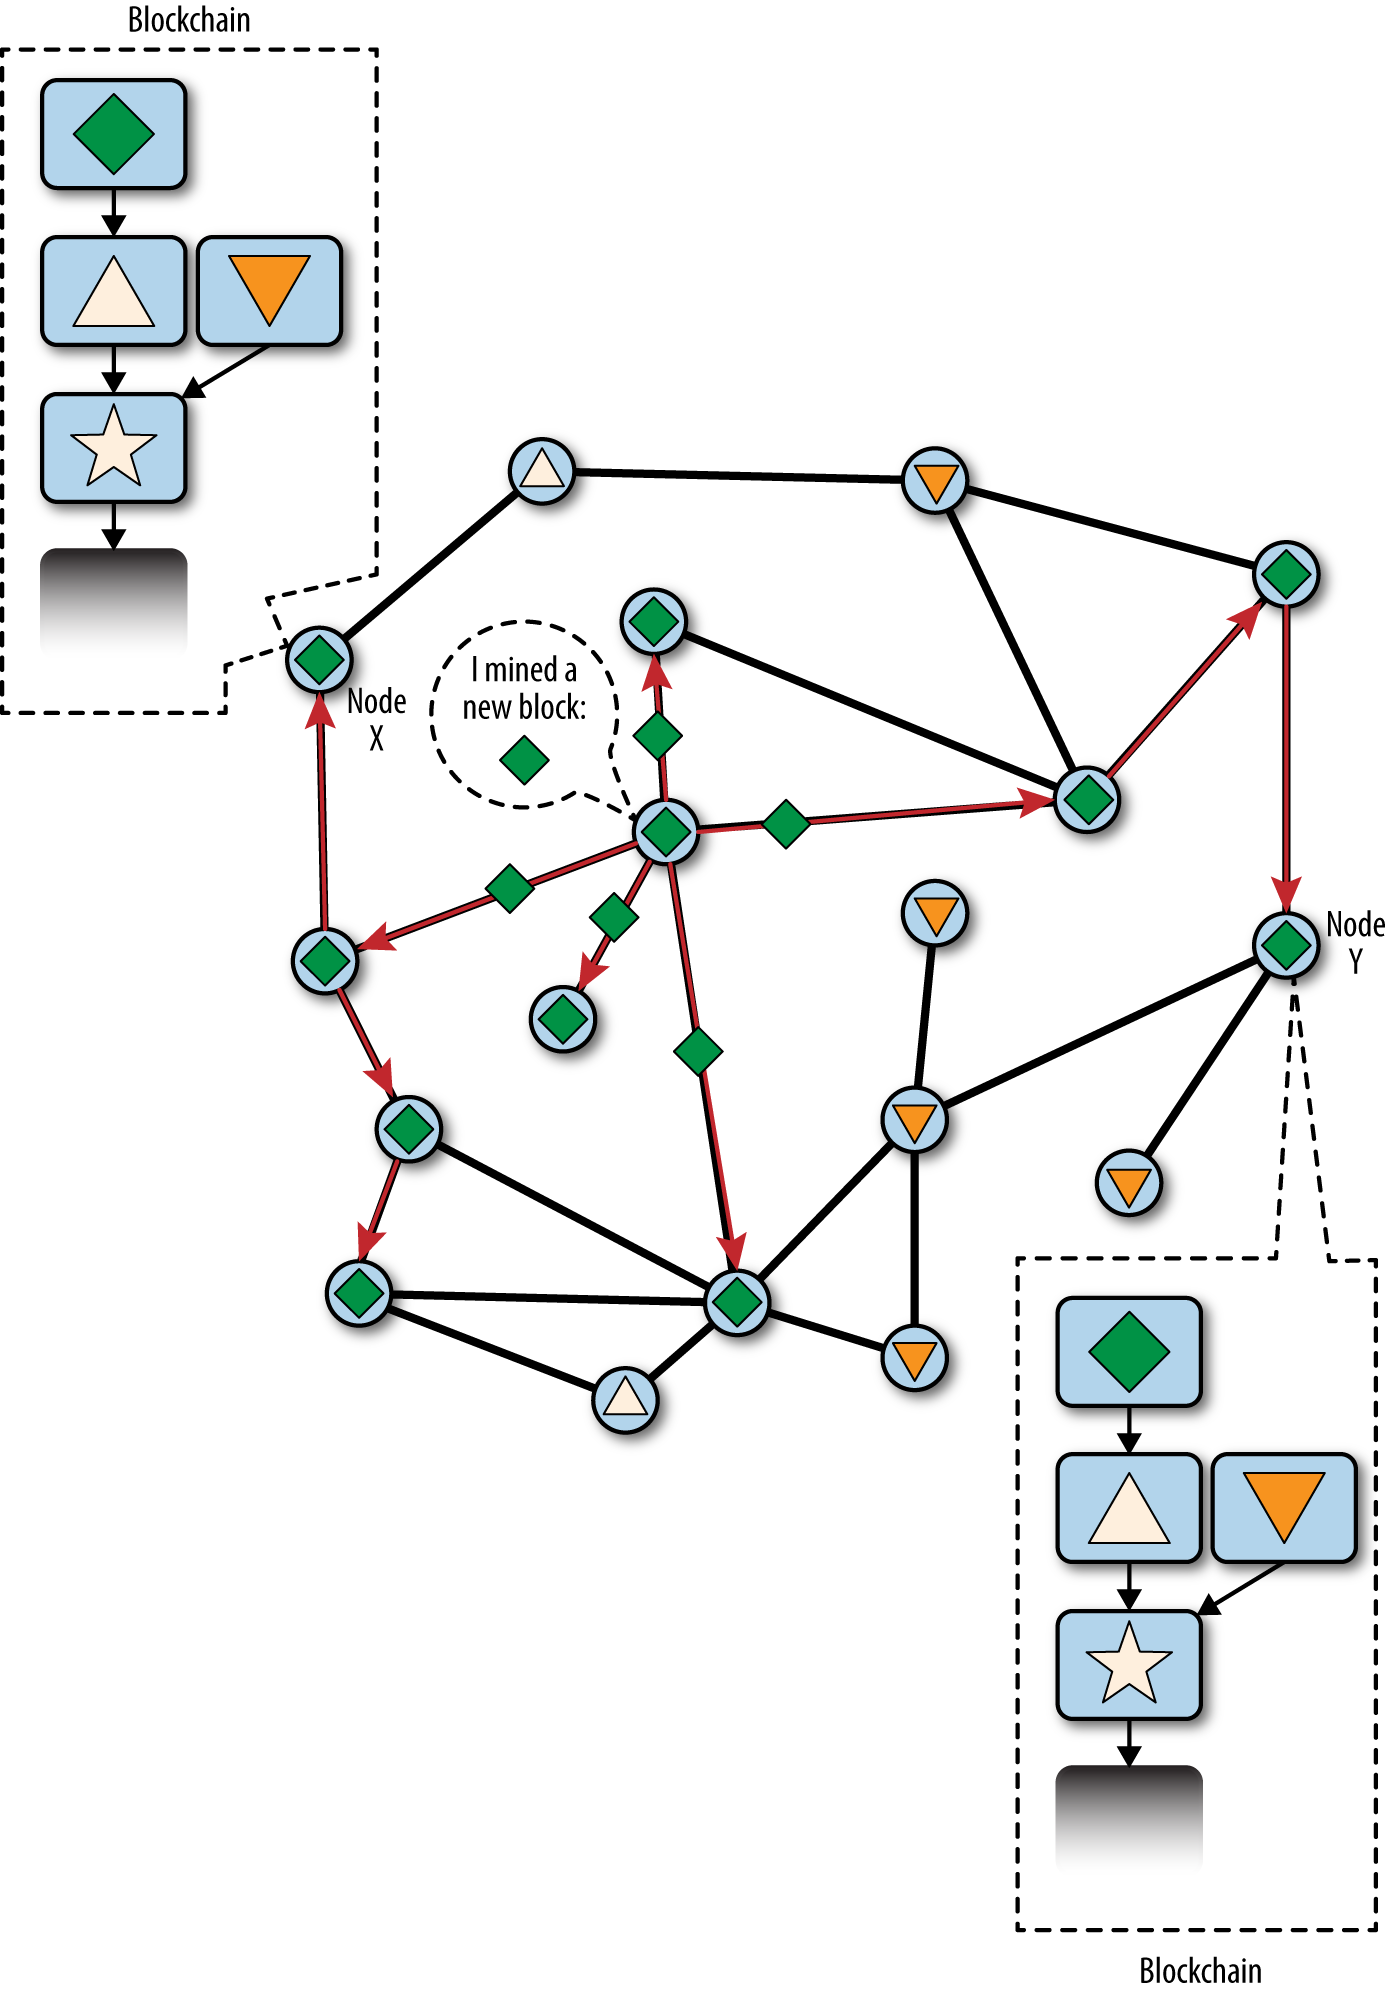
\includegraphics[scale=0.47,clip=false]{pictures/mbc2_1005.png}
  \end{center}

\end{frame}

\begin{frame}\frametitle{Fork: the network reconverges}

  \begin{center}
    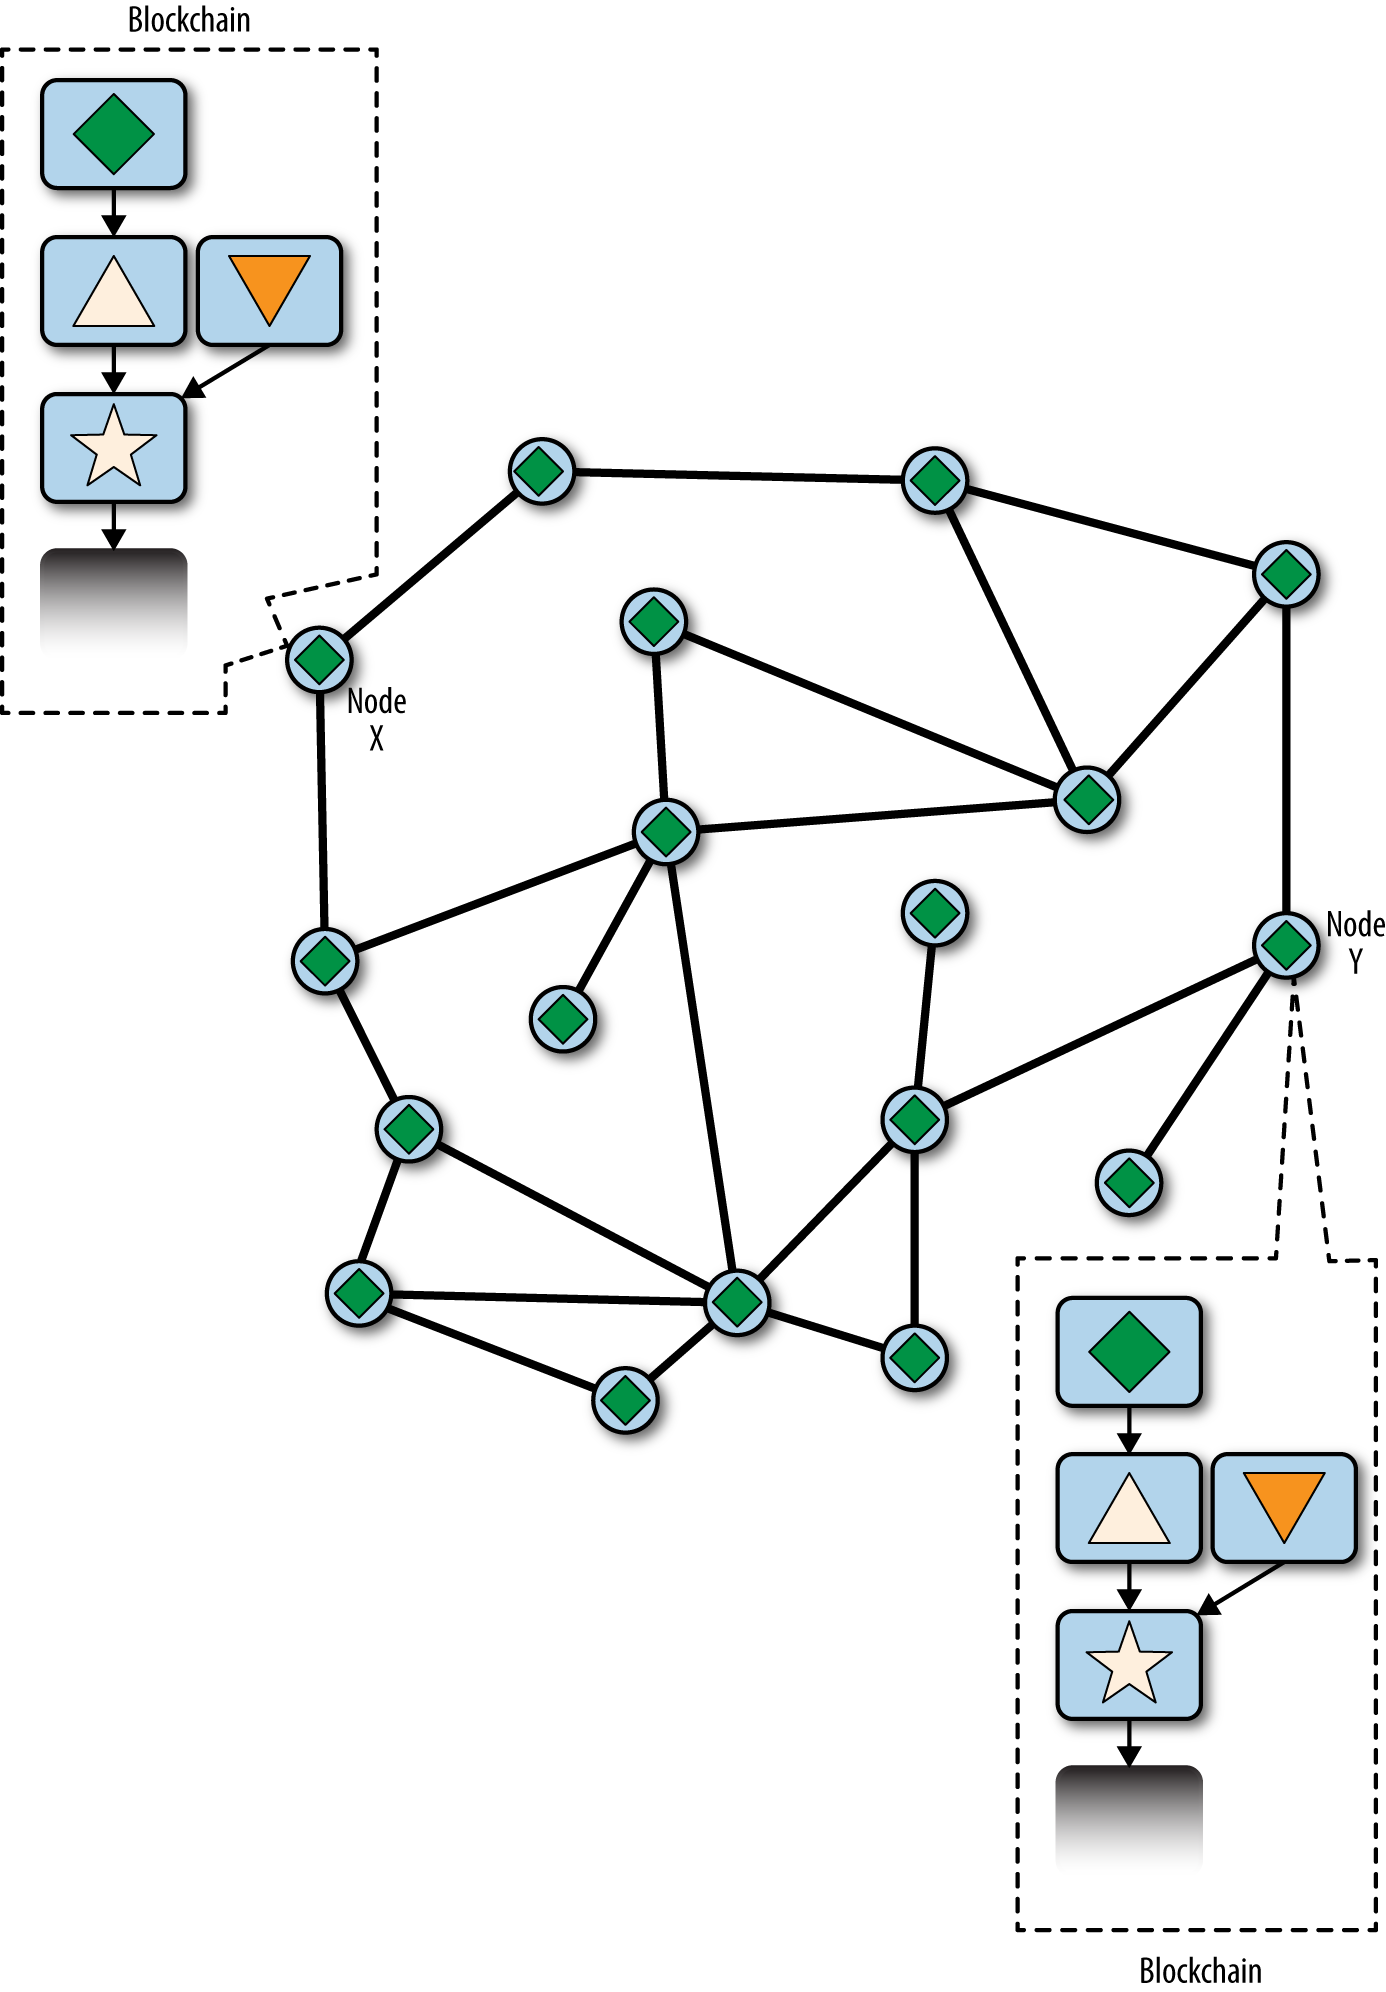
\includegraphics[scale=0.47,clip=false]{pictures/mbc2_1006.png}
  \end{center}

\end{frame}

\begin{frame}\frametitle{State update in case of history change}

    \begin{center}
      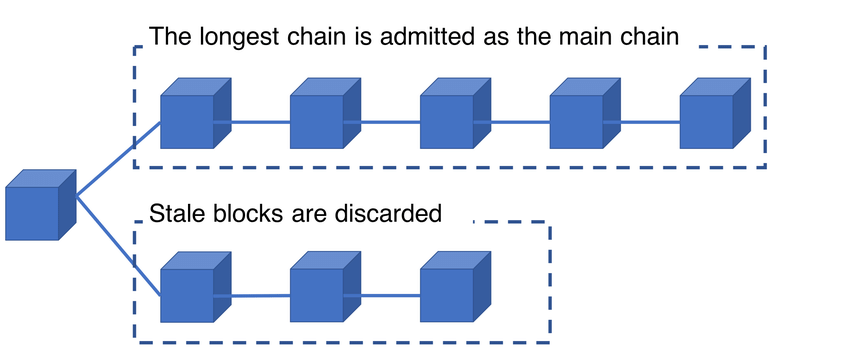
\includegraphics[width=\textwidth,clip=false]{pictures/longest.png}
    \end{center}

    \begin{enumerate}
    \item the transactions in the discarded chain must be undone (easy in Bitcoin)
    \item the transactions in the longest chain must be done (easy)
    \end{enumerate}
    
\end{frame}

\begin{frame}\frametitle{The magic behind PoW}

  \begin{greenbox}{}
    It makes expensive the production of new blocks, in time and cost (electricity)
    \begin{itemize}
    \item who produces invalid blocks sees its blocks rejected by peers and wastes resources
    \item a single node cannot drive the history, since it must fight against
      the hashing power of all other nodes together
    \item forks become unlikely, since the probability of two nodes finding a new block at the same time
      is small
    \end{itemize}
  \end{greenbox}

\end{frame}

\begin{frame}\frametitle{Difficulty over time}

  \begin{center}
    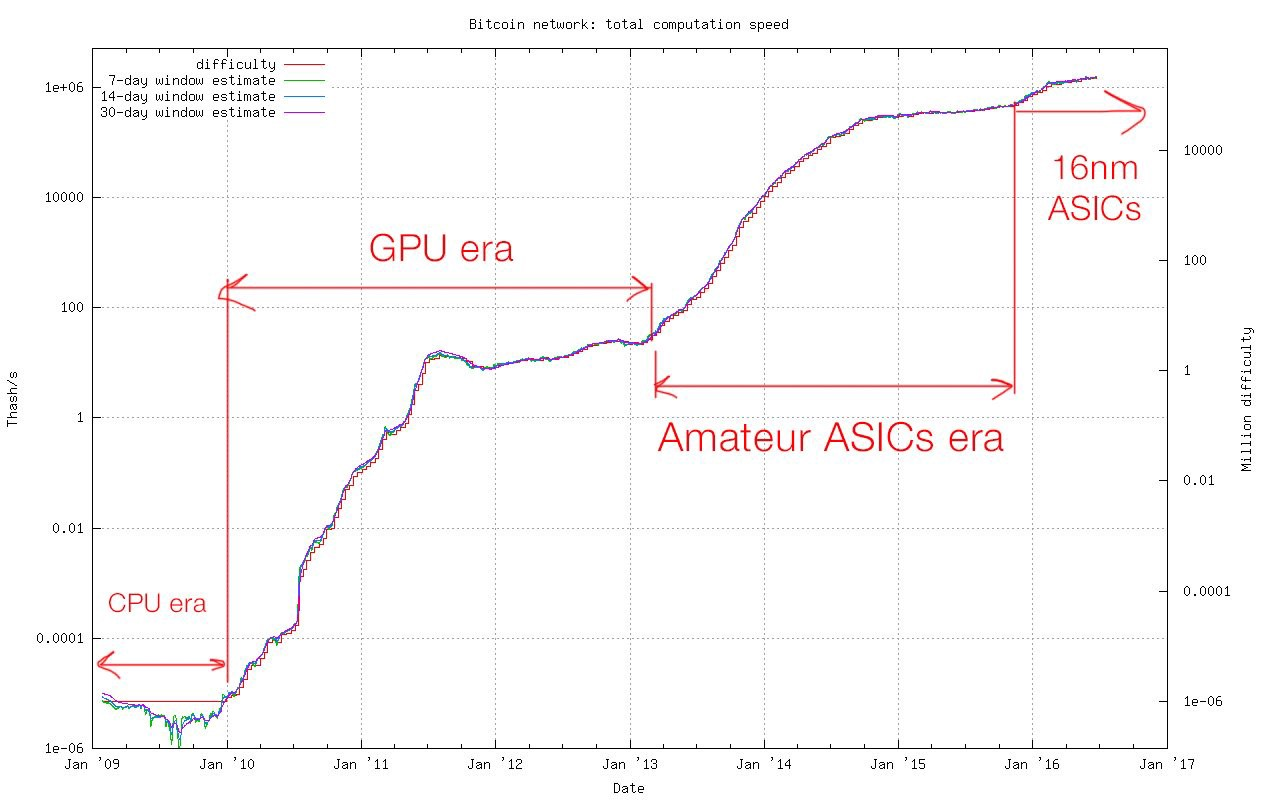
\includegraphics[width=\textwidth,clip=false]{pictures/difficulty.jpg}
  \end{center}

\end{frame}

\begin{frame}\frametitle{PoW costs electricity}

  \begin{greenbox}{2019}
    \begin{center}
      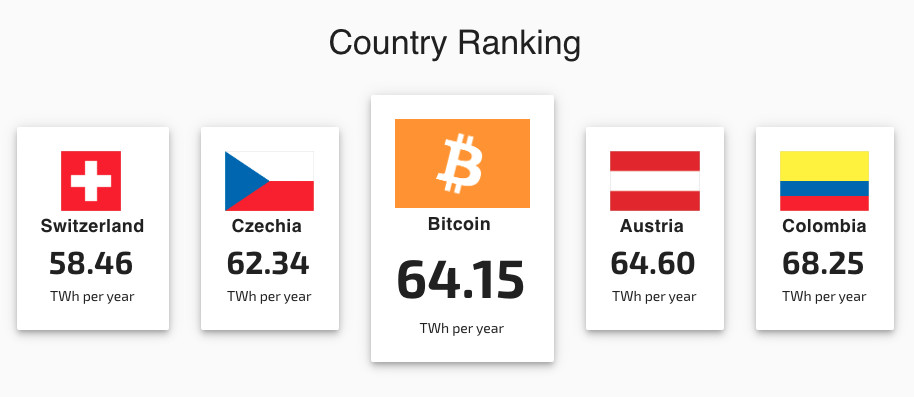
\includegraphics[scale=0.17,clip=false]{pictures/bitcoin-consumption.jpg}
      
\includegraphics[scale=0.14,clip=false]{pictures/greta.jpg}
    \end{center}
  \end{greenbox}
    
\end{frame}

\begin{frame}\frametitle{Consensus attacks}

  \begin{greenbox}{Two main categories}
    \begin{enumerate}
    \item history change (for the topmost few blocks)
    \item denial of service (against specific transactions or accounts)
    \end{enumerate}
  \end{greenbox}

  \bigskip

  Possible if the attacker controls a large portion of the total hashing power

  \begin{center}
    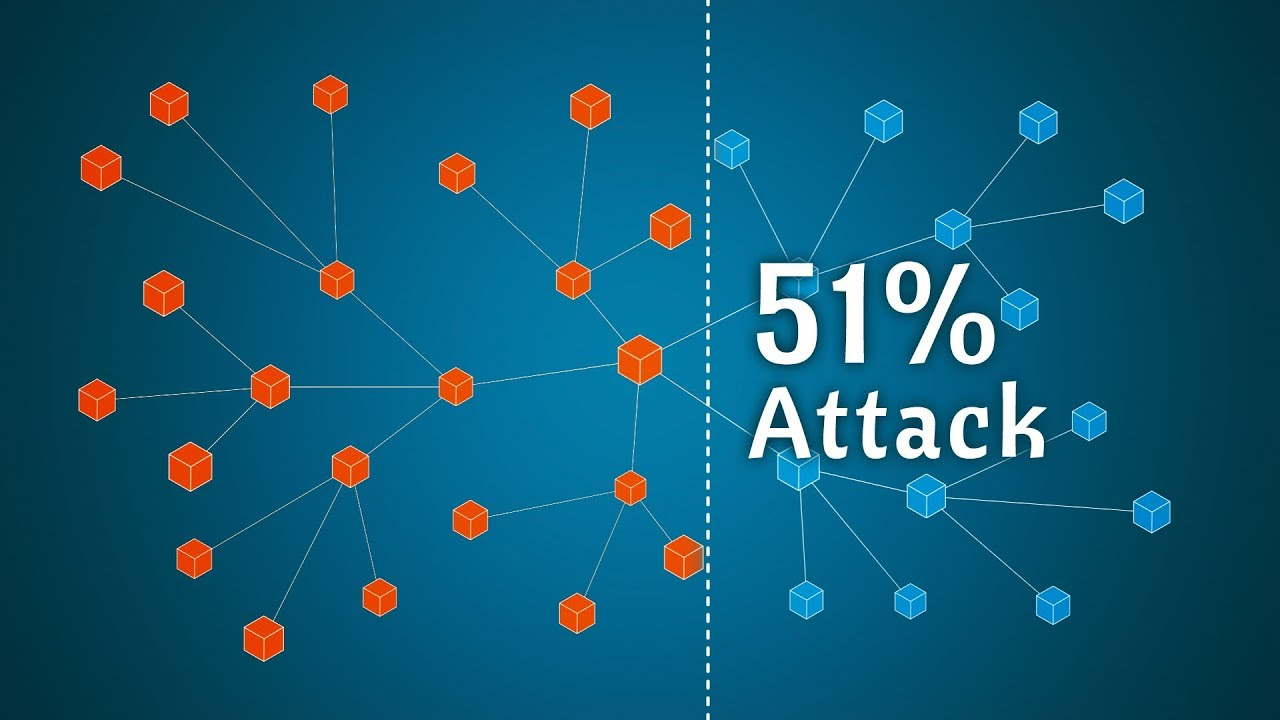
\includegraphics[scale=0.17,clip=false]{pictures/51-percenters.jpg}
  \end{center}

\end{frame}

\begin{frame}\frametitle{Bitcoin has probabilistic finality}

  \begin{center}
    \includegraphics[width=\textwidth,clip=false]{pictures/finality.png}
  \end{center}

\end{frame}

\section{Ethereum}

\begin{frame}
  \frametitle{The world computer}

  \begin{greenbox}{}
    An open source, globally \alert{decentralized computing infrastructure}
    that executes programs called \alert{smart contracts}, written
    in a \alert{Turing-complete} programming language, translated into
    bytecode and run on a \alert{virtual machine}. It uses a
    \alert{blockchain} to synchronize and store the system's \alert{singleton state} changes
    (key/value tuples), along
    with a cryptocurrency called \alert{ether} to \alert{meter and constrain}
    execution resource costs. It enables developers to build
    \alert{decentralized applications} with \alert{built-in economic functions}
  \end{greenbox}

  \begin{center}
    \includegraphics[scale=0.3,clip=false]{pictures/world-computer.jpg}
  \end{center}

\end{frame}

\begin{frame}\frametitle{DApps}

  \begin{greenbox}{DApps = smart contracts (Solidity) + web3 frontend (JavaScript\ldots)}
    \begin{center}
      \includegraphics[scale=0.43,clip=false]{pictures/dapps.png}
    \end{center}
  \end{greenbox}

\end{frame}

\begin{frame}\frametitle{People behind Ethereum}

  \begin{center}
  \begin{tabular}{c@{\hskip 1.5cm}c}
    \includegraphics[scale=.3,clip=false]{pictures/vitalik_buterin.jpg} &
    \includegraphics[scale=.247,clip=false]{pictures/gavin_wood.jpg} \\
    Vitalik Buterin & Gavin Wood
  \end{tabular}
  \end{center}
  
\end{frame}

\begin{frame}\frametitle{Suggested references}

  \begin{center}
    Yellow Paper: \url{https://ethereum.github.io/yellowpaper/paper.pdf}\\
    \mbox{}\\
    \begin{tabular}{c@{\hskip 1cm}c@{\hskip 1cm}c}
      \includegraphics[scale=.25,clip=false]{pictures/mastering-ethereum.jpg} &
      \includegraphics[scale=.25,clip=false]{pictures/building-games.jpg} &
      \includegraphics[scale=.25,clip=false]{pictures/hands-on.jpg}
    \end{tabular}
  \end{center}

  \begin{center}
    The leftmost: \url{https://github.com/ethereumbook/ethereumbook}
  \end{center}

\end{frame}

\begin{frame}\frametitle{Deterministic (infinite) state machine}

  \begin{greenbox}{A very abstract view of blockchain}
    A blockchain is a distributed ledger of transaction requests, aggregated in blocks
    \begin{itemize}
    \item[] \hspace*{-3ex}\alert{Bitcoin:} transaction requests require a change of the set of UTXOs
    \item[] \hspace*{-3ex}\alert{Ethereum:} transaction requests require a change of a
      map $\mathit{key}\to\mathit{value}$
    \end{itemize}
    The change must be \alert{deterministic} otherwise consensus cannot be reached!
  \end{greenbox}

\end{frame}

\begin{frame}\frametitle{Externally owned accounts (EOA) and contracts}

  \begin{greenbox}{}
    EOAs have keys, contracts have code, both have an address
  \end{greenbox}
  
  \begin{center}
    \includegraphics[scale=0.35,clip=false]{pictures/eoa-contract.jpg}
  \end{center}

\end{frame}

\begin{frame}\frametitle{Ethereum transactions}

  \begin{greenbox}{}
    A transaction is a signed message originated by an EOA, transmitted
    by the Ethereum network, and recorded on the Ethereum blockchain:
    \begin{itemize}
    \item nonce: sequence number per each originating EOA
    \item gas price: maximum willing to pay
    \item gas limit: maximum willing to consume
    \item to: recipient (destination address)
    \item value: ether sent to destination
    \item data: generic payload (method name, parameters, contract code\ldots)
    \item signature: ECDSA signature of the originating EOA
    \end{itemize}
  \end{greenbox}

  \begin{center}
    The address of the originating EOA is implied by the signature
  \end{center}

\end{frame}

\begin{frame}\frametitle{Many kinds of transactions}

  \begin{center}
    \includegraphics[width=\textwidth,clip=false]{pictures/many-transactions.png}
  \end{center}

\end{frame}

\begin{frame}\frametitle{The nonce}

  \begin{greenbox}{The nonce of an EOA}
    A scalar value equal to the number of transactions sent from the EOA
  \end{greenbox}

  \bigskip

  \begin{greenbox}{Wallets keep track of nonces}
    They increase it and attach to each transaction they create per
    originating EOA
  \end{greenbox}

  \bigskip

  \begin{greenbox}{Nodes check nonces}
    They count the number $n$ of transactions originated
    by the EOA. If the nonce is smaller than $n+1$, the
    transaction is rejected. If the nonce is greater than $n+1$,
    the transaction is delayed and not yet executed:
    \begin{itemize}
    \item this guarantees transaction ordering
    \item and avoids transaction replaying
    \end{itemize}
  \end{greenbox}

\end{frame}

\begin{frame}\frametitle{Why Ethereum's transactions have a nonce?}

  \begin{greenbox}{Bitcoin's transactions can only transform UTXOs into TXOs}
    It is not possible to spend a UTXO again, inside the same history:
    it would be against the consensus rules
    \begin{itemize}
    \item[$\Rightarrow$] Executing a valid transaction today makes it invalid tomorrow
    \end{itemize}
  \end{greenbox}

  \bigskip
  \bigskip

  \begin{greenbox}{Ethereum's transactions can induce any state change or fail}
    A valid (syntactically correct) transaction can always be executed in Ethereum
    \begin{itemize}
    \item[$\Rightarrow$] Executing a valid transaction today doesn't make it invalid tomorrow
      \alert{(without a nonce)}
    \end{itemize}
  \end{greenbox}

\end{frame}

\begin{frame}\frametitle{The state of Ethereum}

  \begin{center}
    The state of Ethereum is a global singleton map {\color{blue}$\sigma:\mathit{key}\to\mathit{value}$}
  \end{center}

  \bigskip

  \begin{redbox}{The state is not in blockchain!}
    Each node keeps and maintains its own copy in a private database
  \end{redbox}

  \bigskip

  \begin{greenbox}{API of the state}
    \begin{enumerate}
    \item \<value=get(address)>
    \item \<put(address, value)>
    \end{enumerate}
  \end{greenbox}

\end{frame}

\begin{frame}\frametitle{Encoding data into the state}

  \begin{greenbox}{Store the balance of an EOA}
    \begin{center}
      \<put(address\_of\_EOA, balance)>
    \end{center}
  \end{greenbox}

  \bigskip

  \begin{greenbox}{Read the balance of an EOA}
    \begin{center}
      \<get(address\_of\_EOA)>
    \end{center}
  \end{greenbox}

\end{frame}

\begin{frame}\frametitle{Encoding data into the state}

  \begin{greenbox}{EOA installs a smart contract}
    \begin{center}
      \<put(>{\color{blue}$\underbrace{\<hash(address\_of\_EOA, nonce\_of\_EOA)>}_{\mathit{address\ of\ the\ new\ smart\ contract}}$}\<, bytecode\_of\_smart\_contract)>
    \end{center}
  \end{greenbox}

  \bigskip

  \begin{greenbox}{A smart contract writes $v$ into its $n$th instance variable (field)}
    \begin{center}
      \<put(>{\color{blue}$\underbrace{\<hash(address\_of\_smart\_contract, n)>}_{\mathit{address\ of\ the\ n-th\ field}}$}\<, v)>
    \end{center}
  \end{greenbox}

  \bigskip

  \begin{greenbox}{A smart contract reads from its $n$th instance variable (field)}
    \begin{center}
      \<get(>{\color{blue}$\underbrace{\<hash(address\_of\_smart\_contract, n)>}_{\mathit{address\ of\ the\ n-th\ field}}$}\<)>
    \end{center}
  \end{greenbox}

\end{frame}

\begin{frame}\frametitle{The hash of the state}

  \begin{greenbox}{In \alert{Bitcoin}, the header of a block contains the hash \alert{of the transactions} in the block}
    That is, the head of the Merkle tree of transactions. Miners must execute
    the transactions to validate them, since invalid transactions would make the whole block invalid,
    which would make the miner lose money
  \end{greenbox}

  \bigskip

  \begin{greenbox}{In \alert{Ethereum}, the header of a block contains the hash \alert{of the state} at the end of the execution of the transactions in the block}
    Since syntactically correct transactions are always valid, this obliges the miners to execute the transactions
  \end{greenbox}

  \bigskip

  \begin{greenbox}{API of the state}
    \begin{enumerate}
    \item \<value=get(address)>
    \item \<put(address, value)>
    \item \<h=get\_hash()>
    \end{enumerate}
  \end{greenbox}

\end{frame}

\begin{frame}\frametitle{The state of a node must change across different views}

  \begin{center}
    \includegraphics[width=\textwidth,clip=false]{pictures/longest.png}
  \end{center}

  \begin{enumerate}
  \item the transactions in the discarded chain must be undone (hard in Ethereum)
  \item the transactions in the longest chain must be done (easy)
  \end{enumerate}

\end{frame}

\begin{frame}\frametitle{Ethereum = Bitcoin + Git}

  \begin{greenbox}{Undo of state updates, up to the state at the end of an old block}
    \begin{center}
      \<checkout(old\_block.header.state\_hash)>\\
      (possible through a Merkle-Patricia trie)
    \end{center}
  \end{greenbox}

  \bigskip

  \begin{greenbox}{The final API of the state}
    \begin{enumerate}
    \item \<value=get(address)>
    \item \<put(address, value)>
    \item \<h=get\_hash()>
    \item \<checkout(h)>
    \end{enumerate}
  \end{greenbox}

\end{frame}

\section{Smart contracts}

\begin{frame}\frametitle{A smart contract is\ldots}

  \begin{itemize}
  \item a computer program (not \emph{smart} nor \emph{a contract})
  \item immutable
  \item deterministic
  \item operating on restricted data
  \item running on a decentralized world computer
  \end{itemize}

  In Ethereum:
  \begin{itemize}
  \item compiled into EVM bytecode
  \item installed in blockchain
  \item has no keys
  \item its installer gets no automatic privileges
  \item runs after a transaction initiated by an EOA
    \begin{itemize}
    \item or a chain of transactions initiated by an EOA
    \item no parallelism, no background processing
    \end{itemize}
  \item transactions are atomic
  \end{itemize}
  
\end{frame}

\begin{frame}\frametitle{Gavin Wood's Solidity}

  \begin{greenbox}{}
    There are many programming languages for Ethereum smart contracts,
    but Solidity is the de facto standard:
    \begin{itemize}
    \item imperative
    \item vaguely object-oriented
    \item in continuous evolution
    \item \alert{non}-strongly-typed
    \item unorthogonal features
    \end{itemize}
  \end{greenbox}

  \bigskip

  \begin{greenbox}{}
    \begin{itemize}
    \item[{\includegraphics[scale=0.03]{pictures/check.png}}] sequence
    \item[{\includegraphics[scale=0.03]{pictures/check.png}}] conditional
    \item[{\includegraphics[scale=0.03]{pictures/check.png}}] repetition
    \end{itemize}

    \begin{center}
      \alert{$\Rightarrow$ Turing complete (bug or feature?)}
    \end{center}

  \end{greenbox}

\end{frame}

\begin{frame}\frametitle{A simple Solidity example}
  \begin{center}
    \includegraphics[width=\textwidth,clip=false]{pictures/faucet_sol.png}
  \end{center}
\end{frame}

\begin{frame}\frametitle{Basic Solidity types}
  \begin{greenbox}{\<bool>}
    with constants \<true> and \<false> and usual operators
  \end{greenbox}
  \bigskip
  \begin{greenbox}{\<int>, \<uint>}
    signed or unsigned, with usual operators, in increments of 8 bit size:
    \<uint8>, \<uint16>, \<int24>\ldots. Without specification, they stand for
    \<int256> and \<uint256>, respectively
  \end{greenbox}
  \bigskip
  \begin{greenbox}{\<fixed>$M\times N$, \<ufixed>$M\times N$}
    fixed point arithmetic, signed or unsigned, $M$ bits, $N$ decimals
    after the point: \alert{currently not implemented}
  \end{greenbox}

\end{frame}

\begin{frame}[fragile]\frametitle{Basic Solidity types}

  \begin{greenbox}{\<bytes>$N$}
    fixed-size array of bytes, of length $N$
  \end{greenbox}

  \bigskip

  \begin{greenbox}{\<bytes> or \<string>}
    variable-sized arrays of bytes
  \end{greenbox}

  \bigskip

  \begin{greenbox}{Arrays}
    \<uint32[][5]> is a fixed size array of five dynamic
    arrays of $32$ bits unsigned integers
  \end{greenbox}

  \bigskip

  \begin{greenbox}{Enumerations}
\begin{verbatim}
enum NAME { A, B, ... }
\end{verbatim}
  \end{greenbox}

\end{frame}

\begin{frame}[fragile]\frametitle{Basic Solidity types}

  \begin{greenbox}{Structures}
\begin{verbatim}
struct pair {
  int16 x;
  uint8 y;
}
\end{verbatim}
  \end{greenbox}

  \medskip

  \begin{greenbox}{Mappings}
\begin{verbatim}
mapping(address => uint256) balances;
\end{verbatim}

A field of type mapping spreads its values into the state through hashing:
\<balances[k]=v> executes
\<put(>{{\color{blue}$\underbrace{\<hash(balances,k)>}_{\mathit{address\ of\ \<balances[k]>}}$}}\<, v)>

\begin{itemize}
\item[$\Rightarrow$] mappings default to $0$
\item[$\Rightarrow$] there is no \<containsKey> (you need a sentinel value)
\item[$\Rightarrow$] it is not possible to compute the key set or value set of a mapping
\item[$\Rightarrow$] it is not possible to iterate on a mapping
\end{itemize}
  \end{greenbox}

\end{frame}

\begin{frame}\frametitle{A simple Ponzi scheme}

  \begin{center}
    \includegraphics[width=\textwidth,clip=false]{pictures/simple-ponzi.png}
  \end{center}

  \begin{center}
    The first investment will be burned to address \<0x0>
  \end{center}
  
\end{frame}

\begin{frame}\frametitle{Gas consumption}

  \begin{greenbox}{Each bytecode instruction and transaction type has a gas cost}
    \begin{itemize}
    \item it is possible to compute in advance the gas cost \alert{of simple functions}
      (use \<estimateGas> in the web3 library for instance)
    \item \alert{the result is wrong in the presence of loops or recursion!}
      \begin{itemize}
      \item obvious, since gas cost computation is harder than complexity analysis
        which can be used to decide termination of programs
        \begin{itemize}
        \item[$\Rightarrow$] an algorithm for computing gas costs in advance cannot exist
        \end{itemize}
      \end{itemize}
    \item in general, it is important to know which operations (might) cost much gas, and avoid them
      \begin{itemize}
      \item loops over unbounded dynamic arrays
      \item calls to unknown contracts
      \end{itemize}
    \end{itemize}
  \end{greenbox}
\end{frame}

\begin{frame}\frametitle{A gradual Ponzi scheme}

  \begin{center}
    \includegraphics[scale=0.4,clip=false]{pictures/gradual-ponzi.png}
  \end{center}

\end{frame}

\begin{frame}\frametitle{Type \<address>: Solidity is \alert{not} strongly-typed}

  \begin{enumerate}
  \item casts are not checked
  \item parameter types are just Christmas decorations
  \end{enumerate}

  \bigskip

  \begin{redbox}{}
    A function declaring a formal parameter of type
    \<address> or explicitly \<C> can actually receive any value, of any
    type, also completely unrelated to \<C>. No run-time error occurs.
    Callers can inject malicious code through such parameters!
    \begin{center}
      \textbf{Never talk to strangers!}
    \end{center}
  \end{redbox}

  \begin{center}
    \includegraphics[scale=0.22,clip=false]{pictures/frightened-cat.jpg}
  \end{center}

\end{frame}

\begin{frame}\frametitle{The DAO attack (2016): they talked to strangers\ldots}

  \begin{center}
    \includegraphics[width=\textwidth,clip=false]{pictures/re-entrancy.png}
  \end{center}

\end{frame}

\begin{frame}\frametitle{The DAO attack (2016)}

  \begin{greenbox}{The most famous reentrancy exploit}
    \begin{itemize}
    \item the DAO was a contract for autonomous decentralized organizations
    \item the attacker used reentrancy to steal $50\text{M}\$$ equivalent of ETH
    \item the Ethereum team decided to make the consensus rules more restrictive in order
      to make such transactions illegal and get some of that money back
    \item some node maintainers didn't accept the change and continued
      operating with the old rules and another chain id, leading to a network hard fork known as
      Ethereum Classic
    \end{itemize}
  \end{greenbox}

  \begin{center}
    \includegraphics[scale=0.5,clip=false]{pictures/ethereum-vs-ethereum-classic.jpg}
  \end{center}

\end{frame}

\begin{frame}\frametitle{Security best practice}

  \begin{itemize}
  \item Minimalism: the simpler, the better
  \item Code reuse: DRY, use well-known libraries
  \item Study: be aware of well-known issues and solutions
  \item Readability: simpler audit
  \item Test: try corner cases
  \item Analysis: static or dynamic, still in infancy
  \end{itemize}

  \bigskip

  \begin{redbox}{}
    Considering the importance of security for smart contracts,
    it is questionable to have invented Solidity (hard, new, weakly-typed,
    complex low-level semantics) for writing such delicate pieces of software
  \end{redbox}

\end{frame}

\section{Tendermint}

\begin{frame}
  \frametitle{Proof of\ldots}

  \begin{center}
    Who decides the next block?
  \end{center}

  \bigskip

  \begin{greenbox}{}
    \begin{itemize}
    \item Proof of work [PoW] (who works harder and is lucky)
    \item proof of stake [PoS] (who commits more money)
    \item proof of space (who commits more disk space)
    \item proof of authority (who has more authority)
    \item \ldots
    \end{itemize}
  \end{greenbox}

  \bigskip

  \begin{greenbox}{PoS is a variant of Practical Byzantine Fault Tolerance (BFT)}
    Miguel Castro and Barbara Liskov.
    \emph{Practical Byzantine Fault Tolerance and Proactive Recovery}.
    ACM Trans.\ Comput.\ Syst., 20(4):398–461, November 2002
  \end{greenbox}

\end{frame}

\begin{frame}\frametitle{Tendermint (now Ignite): \url{ignite.com}}

  \begin{greenbox}{Jae Kwon. \emph{Tendermint: Consensus without Mining}, 2014.\\
    \url{https://tendermint.com/static/docs/tendermint.pdf}}
    \begin{itemize}
    \item a dynamic set $V$ of validators decides the next block
    \item $V$ might be different for each block
      \begin{itemize}
      \item but deterministically computed from the previous history
      \end{itemize}
    \item at each height $H$, each validator $v\in V$:
      \begin{enumerate}
      \item identifies (deterministically) a validator $p\in V$ that
        is expected to aggregate some transactions and that \alert{proposes} a next block $b$
      \item if $v$ considers $b$ valid, it \alert{pre-votes} $b$
      \item $v$ counts how many validators pre-voted $b$
      \item if $v$ counted at least $\frac{2}{3}$ pre-votes, $v$ \alert{pre-commits} $b$
      \item $v$ counts how many validators pre-committed $b$
      \item if $v$ counted at least $\frac{2}{3}$ pre-commits, $v$ \alert{commits} $b$ and increases $H$
      \item $v$ goes back to step~1
      \end{enumerate}
    \end{itemize}
  \end{greenbox}

  \smallskip

  \begin{center}
    Tendermint is BFT. If step~1 or rewards are based on stakes, then it is PoS
  \end{center}

\end{frame}

\begin{frame}\frametitle{Inside a Tendermint block}

  \begin{center}
    \includegraphics[scale=.38,clip=false]{pictures/tendermint-block.png}
  \end{center}

\end{frame}

\begin{frame}\frametitle{Proof of stake: can we trust it?}

  \begin{greenbox}{Yes we can: Ethereum successfully moved from PoW to PoS}
    \begin{itemize}
    \item it's a special case, whose coin is very valuable: validators are a serious form of investment
    \end{itemize}
  \end{greenbox}

  \bigskip
  
  \begin{redbox}{No we can't: all new blockchain projects use PoS nowadays}
    \begin{itemize}
    \item validators have no interest in being validators (the coin has no value)
    \item validators are afraid of having a machine always connected and open to the internet
    \item validators find it expensive to maintain and update their machine
    \item validators lose cryptocurrency if a blackout or network failure isolate their machine
    \item please ask this question: ``How many validators your blockchain project has, where are they and who maintains such machines'' (spoiler: very few, in the same room, all maintained by a single person)
    \end{itemize}
  \end{redbox}

\end{frame}

\begin{frame}\frametitle{A layered implementation in Golang}

  \begin{center}
    \includegraphics[scale=.45,clip=false]{pictures/tendermint-core.jpg}
  \end{center}

  \begin{center}
    ABCI: Application BlockChain Interface
  \end{center}

\end{frame}

\begin{frame}\frametitle{The ABCI}

  \begin{center}
    \url{https://docs.tendermint.com/master/spec/abci/abci.html}
  \end{center}

  \begin{itemize}
  \item[] \alert{\<checkTx>}: called before entering the mempool and to verify blocks
    \begin{itemize}
    \item[$\Rightarrow$] only transactions that satisfy \<checkTx> are added in blocks
    \item[{\includegraphics[scale=0.0135]{pictures/uncheck.png}}] must not modify the state of the application
    \end{itemize}
    \hrule
  \item[] \alert{\<beginBlock>}: called at the beginning of a block; receives information
    about the validator set of the previous block and which of them signed the previous block
  \item[] \alert{\<deliverTx>}: called for each transaction added to a block: it executes
    the transaction by modifying the state of the application
  \item[] \alert{\<endBlock>}: called at the end of a block; provides information
    about the validator set for the next block
  \item[] \alert{\<commit>}: called when a block is being committed; provides the hash of
    the state of the application
    \hrule
  \item[] \alert{\<query>}: called when the user wants to read data from the blockchain
  \end{itemize}
\end{frame}

\begin{frame}\frametitle{The database of blocks and the application state}

  \begin{center}
    \includegraphics[width=\textwidth,clip=false]{pictures/tendermint-databases.png}
  \end{center}

\end{frame}

\begin{frame}\frametitle{The application state}

  \begin{greenbox}{It must have a function to compute its hash}
    Only that hash is reported in blockchain, for consensus
  \end{greenbox}

  \bigskip

  \begin{greenbox}{It must allow transactional, atomic updates}
    Between \<beginBlock> and \<commit>
  \end{greenbox}

  \bigskip

  \begin{greenbox}{The API of the state}
    Tendermint enjoys finality: there are no forks
    \begin{itemize}
      \item[$\Rightarrow$] one never needs to come
        back in time to the state of a previous block
    \end{itemize}

    \begin{enumerate}
    \item get data
    \item put data
    \item \<h=get\_hash()>
    \item \sout{\<checkout(h)>} $\Rightarrow$ big opportunity for garbage collection!
    \end{enumerate}
  \end{greenbox}

\end{frame}

\begin{frame}\frametitle{Cosmos: a Tendermint application in Golang}

  \begin{center}
    \includegraphics[scale=0.2,clip=false]{pictures/cosmos.png}
  \end{center}

\end{frame}

\section{Hotmoka + Takamaka}

\begin{frame}
  \frametitle{Hotmoka (Fausto Spoto, 2019--2021): \url{www.hotmoka.io}}

  \begin{center}
    \includegraphics[scale=0.2,clip=false]{pictures/hotmoka_logo.png}
  \end{center}
  
  \begin{greenbox}{}
    An open-source implementation of a network of nodes:
    \begin{itemize}
    \item nodes of a blockchain
    \item IoT devices
    \item computers in the cloud
    \end{itemize}
  \end{greenbox}

  \bigskip

  \begin{greenbox}{Requests are OO-based}
    \begin{itemize}
    \item install code in the node
    \item create an object
    \item call a method of an object
    \item methods are implemented in Takamaka (subset of Java)
    \end{itemize}
  \end{greenbox}

\end{frame}

\begin{frame}\frametitle{Hotmoka nodes \underline{can} be Tendermint applications}

  \begin{center}
    \includegraphics[width=\textwidth,clip=false]{pictures/tendermint-databases.png}
  \end{center}
    
\end{frame}

\begin{frame}\frametitle{An OO state (hash is sha256)}

  \begin{center}
    \includegraphics[width=\textwidth,clip=false]{pictures/hotmoka-structure.pdf}
  \end{center}

\end{frame}

\begin{frame}[fragile]\frametitle{The state contains actual Java objects}

  {\scriptsize
    \texttt{manifest:} $\underbrace{{\color{red}\mathtt{42a8a11aee0405aee5775514b3b0456c7740bbb015b4b87df4776e6e4add7668\#0}}}_{\text{machine-independent memory address of an object}}$
  }

  \bigskip

  \begin{greenbox}{{\scriptsize\<moka state 42a8a11aee0405aee5775514b3b0456c7740bbb015b4b87df4776e6e4add7668\#0 --url panarea.hotmoka.io>}}
    {\tiny\begin{semiverbatim}
class {\color{violet}io.takamaka.code.governance.Manifest} (from jar installed at 02dfd29348abaa44f7205251...)
  allowsSelfCharged:boolean = false
  allowsUnsignedFaucet:boolean = true
  chainId:java.lang.String = "chain-ASdWiN"
  gamete:io.takamaka.code.lang.Account = {\color{red}4f7d7ca1fbea152d8f323c21e1abcfa1d979c7c4ea667d8457381a26b08a2d71#0}
  gasStation:io.takamaka.code.governance.GasStation = {\color{red}42a8a11aee0405aee5775514b3b0456c7740bbb015b4b8...}
  maxCumulativeSizeOfDependencies:long = 10000000
  maxDependencies:int = 20
  maxErrorLength:int = 300
  signature:java.lang.String = "ed25519"
  skipsVerification:boolean = false
  validators:io.takamaka.code.governance.Validators = {\color{red}42a8a11aee0405aee5775514b3b0456c7740bbb015b4b8...}
  versions:io.takamaka.code.governance.Versions = {\color{red}42a8a11aee0405aee5775514b3b0456c7740bbb015b4b87df4...}
^ balance:java.math.BigInteger = 0 {\color{violet}(inherited from io.takamaka.code.lang.Contract)}
^ balanceRed:java.math.BigInteger = 0 {\color{violet}(inherited from io.takamaka.code.lang.Contract)}
^ nonce:java.math.BigInteger = 227 {\color{violet}(inherited from io.takamaka.code.lang.ExternallyOwnedAccount)}
^ publicKey:java.lang.String = "" {\color{violet}(inherited from io.takamaka.code.lang.ExternallyOwnedAccount)}
    \end{semiverbatim}}
  \end{greenbox}

\end{frame}

\begin{frame}[fragile]\frametitle{How can Hotmoka identify updates to fields of objects?}

  \begin{greenbox}{The original code}
    \begin{semiverbatim}
      public class C \{
        public {\color{blue}int i;}
        public void foo() \{
          {\color{blue}i} = 42;
        \}
      \}
    \end{semiverbatim}
  \end{greenbox}

  \begin{center}
    No way to know if \<i> changed its value during the execution of \<foo()>
  \end{center}

\end{frame}

\begin{frame}[fragile]\frametitle{How can Hotmoka identify updates to fields of objects?}

  \begin{greenbox}{The instrumented code}
    \begin{semiverbatim}
      public class C {\color{red}extends Storage} \{
        public {\color{blue}int i, old\_i;} // aliased at method start
        public void foo() \{
          {\color{blue}i} = 42;
        \}
      \}
    \end{semiverbatim}
  \end{greenbox}

  \begin{center}
    \<i> changed its value during the execution of \<foo()> iff at the end \<i>$\not=$\<old\_i>
  \end{center}

\end{frame}

\begin{frame}[fragile]\frametitle{How can Hotmoka enforce gas limits?}

  \begin{greenbox}{The original code}
    \begin{semiverbatim}
      public class C \{
        public void foo() \{
          while (...) \{
            ...
          \}
        \}
      \}
    \end{semiverbatim}
  \end{greenbox}

  \begin{center}
    This loop might run for very long or even forever
  \end{center}

\end{frame}

\begin{frame}[fragile]\frametitle{How can Hotmoka enforce gas limits?}

  \begin{greenbox}{The instrumented code}
    \begin{semiverbatim}
      {\color{blue}static long counter;}
      public class C \{
        public void foo() \{
          while (...) \{
            {\color{blue}if (counter++ >= gaslimit)
              throw new OutOfGasError();}
            ...
          \}
        \}
      \}
    \end{semiverbatim}
  \end{greenbox}

  \begin{center}
    Actual gas costs are more fine-grained
  \end{center}

\end{frame}

\begin{frame}\frametitle{Verification and instrumentation of jars in state}

  Each jar that gets installed in a Hotmoka node undergoes two processes:

  \begin{enumerate}
  \item Verification: absence of frequent errors
    \begin{itemize}
    \item objects stored in state extend \<Storage>
    \item non-deterministic or non-terminating library code is not used
    \item no synchronization
    \item no native code
    \item no \emph{dangerous} bytecodes
    \item no finalizers
    \item no static fields (mostly)
    \item code annotations are used correctly
    \item \ldots
    \end{itemize}
  \item Instrumentation
    \begin{itemize}
    \item fields of \<Storage> classes get duplicated
    \item gas metering is weaved into the code
    \item code annotations get implemented \emph{by magic}
    \item \<caller()> is given semantics
    \item \ldots
    \end{itemize}
  \end{enumerate}

\end{frame}

\begin{frame}\frametitle{The Takamaka programming language}

  Takamaka is the subset of Java that passes the verification
  of a Hotmoka node. It uses code annotations to implement contract-based aspects:

  \begin{itemize}
  \item {\color{blue}\<@FromContract>} annotates something that can only be called by a contract,
    not by any other code; hence, it has a {\color{blue}\<caller()>}
  \item {\color{blue}\<@Payable>} annotates something whose execution requires to pay some
    cryptocurrency units
  \item {\color{blue}\<@View>} annotates something whose execution can be run for free,
    without paying for its gas: it must not generate any update at its end
    (\emph{pure} code)
  \end{itemize}

  \bigskip
  Takamaka comes equipped with a {\color{blue}support library}
  (\<io-takamaka-code>) that defines such annotations and
  other typical classes that are useful
  for programming smart contracts (tokens, NFTs, DAOs)

\end{frame}

\begin{frame}[fragile]\frametitle{An example of a Takamaka smart contract}

\vspace*{-1ex}{\tiny\begin{semiverbatim}
{\color{darkblue}{
import static io.takamaka.code.lang.Takamaka.require;
import java.math.BigInteger;
import io.takamaka.code.lang.Contract;
import io.takamaka.code.lang.FromContract;
import io.takamaka.code.lang.Payable;
import io.takamaka.code.lang.PayableContract;
import io.takamaka.code.lang.View;

public class SimplePonzi {\color{red}extends Contract} \{
  private final BigInteger _10 = BigInteger.valueOf(10L), _11 = BigInteger.valueOf(11L);
  private {\color{armygreen}PayableContract} currentInvestor;
  private BigInteger currentInvestment = BigInteger.ZERO;

  public {\color{violet}@Payable} {\color{armygreen}@FromContract(PayableContract.class)} void invest({\color{violet}BigInteger amount}) \{
    BigInteger minimum = currentInvestment.multiply(_11).divide(_10);
    require(amount.compareTo(minimum) >= 0, () -> "you must invest at least " + minimum);

    if (currentInvestor != null)
      currentInvestor.{\color{armygreen}receive(amount)}; {\color{red}// no risk of reentrancy}

    currentInvestor = {\color{armygreen}(PayableContract) caller()};
    currentInvestment = amount;
  \}

  public {\color{red}@View} BigInteger getCurrentInvestment() \{
    return currentInvestment;
  \}
\}
}}\end{semiverbatim}}

\end{frame}

\begin{frame}[fragile]\frametitle{An insurance smart contract in Takamaka}

  \begin{greenbox}{The contract allows one to insure specific days of the year}
    If it rains on those days, one will get an indemnization larger than
    the cost of the insurance
    \begin{itemize}
    \item much larger in summer
    \item just a bit larger in winter
    \end{itemize}
  \end{greenbox}

  \medskip
  The contract provides the following functionalities:

  \begin{itemize}
  \item construction, upon specification of the oracle:
    \[\<{\color{violet}@FromContract} {\color{airforceblue}@Payable} Insurance({\color{airforceblue}BigInteger amount}, Contract oracle)>\]
  \item purchase of an insurance for specific days:
    \[\<{\color{violet}@FromContract(PayableContract.class)} {\color{airforceblue}@Payable} void buy>\]
    \vspace*{-5ex}
    \[\<({\color{airforceblue}long amount}, int day, int month, int year, int duration)>\]
  \item notification of rain and indemnization:
    \[\<{\color{violet}@FromContract} void itRains()>\]
  \end{itemize}
\end{frame}

\begin{frame}[fragile]\frametitle{An insurance contract}

  {\scriptsize\begin{semiverbatim}
public class Insurance extends {\color{blue}Contract} \{
  public final static long MIN = 1_000, MAX = 1_000_000_000;
  private final {\color{blue}Contract} oracle;
  private final {\color{blue}StorageSet}<InsuredDay> insuredDays = new {\color{blue}StorageTreeSet<>()};

  public {\color{violet}@FromContract} {\color{airforceblue}@Payable} Insurance({\color{airforceblue}BigInteger amount}, Contract oracle) \{
    this.oracle = oracle;
  \}

  {\color{red}// inner class}
  private static class InsuredDay extends {\color{blue}Storage} \{ {\color{red}/* not shown */} \}

  public {\color{violet}@FromContract(PayableContract.class)} {\color{airforceblue}@Payable} void buy
    ({\color{airforceblue}long amount}, int day, int month, int year, int duration) \{ {\color{red}/* shown later */} \}

  public {\color{violet}@FromContract} void itRains() \{ {\color{red}/* shown later */} \}
\}
  \end{semiverbatim}}

\end{frame}

\begin{frame}[fragile]\frametitle{Buy an insurance}

{\scriptsize\begin{semiverbatim}
public {\color{violet}@FromContract(PayableContract.class)} {\color{airforceblue}@Payable} void buy
    ({\color{airforceblue}long amount}, int day, int month, int year, int duration) \{

  {\color{armygreen}require(duration >= 1, "you must insure at least one day");
  require(duration <= 7, "you cannot insure more than a week");
  require(amount >= MIN * duration,
    () -> "we insure a single day for at least " + MIN + " units of coin");
  require(amount <= MAX * duration,
    () -> "we insure a single day for up to " + MAX + " units of coin");}

  // if the date is wrong, this generates an exception
  LocalDate start = LocalDate.of(year, month, day);

  PayableContract payer = (PayableContract) {\color{violet}caller()};
  for (int offset = 0; offset < duration; offset++)
    insuredDays.add(new InsuredDay
                    (payer, amount / duration, start.plusDays(offset)));
\}
\end{semiverbatim}}

\end{frame}

\begin{frame}[fragile]\frametitle{Pay the indemnization}

{\scriptsize\begin{semiverbatim}
public {\color{violet}@FromContract} void itRains() \{
  {\color{armygreen}require({\color{violet}caller()} == oracle, "only the oracle can call this method");}

  {\color{red}// pay who insured today}
  insuredDays.stream()
    .filter(InsuredDay::isToday)
    .forEachOrdered(insuredDay ->
          insuredDay.payer.{\color{blue}receive}(insuredDay.indemnization()));

  {\color{red}// clean-up the set of insured days}
  insuredDays.stream()
    .filter(InsuredDay::isTodayOrBefore)
    .forEachOrdered(insuredDays::remove);
\}
\end{semiverbatim}}

\end{frame}

%moka install 251bfca0a37c0cc2611f3a5caee95fedb972e820609c6a0912d2527af53f59bb#0 target/insurance-0.0.1.jar --url panarea.hotmoka.io
\begin{frame}[fragile]\frametitle{On-chain verification: incorrect use of annotations}

  \begin{redbox}{Assume that the programmer forgets the \<FromContract> annotation in \<buy>}
  \<public {\color{green}\sout{@FromContract(PayableContract.class)}} @Payable void buy
  (long amount, int day, int month, int year, int duration)>
  \end{redbox}\pause

  \begin{tt}mvn clean package\end{tt} $\Rightarrow$ regenerates \<target/insurance-0.0.1.jar>\pause

\medskip

\begin{greenbox}{Let's try to install this version of the jar}
{\scriptsize\begin{semiverbatim}
 {\color{red}moka install
 06aa6a1afabc82c7161ffcdc2391a2136101aaeb94f64edd53a1d0d1436d610e\#0
 target/insurance-0.0.1.jar
 --url panarea.hotmoka.io}\pause

Do you really want to spend up to 852500 gas units to install the jar [Y/N] Y
{\color{armygreen}total gas consumed: 852500}
{\color{darkred}  for CPU: 255
  for RAM: 1326
  for storage: 381762
  for penalty: 469157     !!!!!!!}
io.hotmoka.beans.TransactionException:
io.takamaka.code.verification.VerificationException:
{\color{red}it/univr/insurance/Insurance.java method buy:
@Payable can only be applied to a @FromContract method or constructor}
\end{semiverbatim}}
\end{greenbox}

\end{frame}

%moka install 251bfca0a37c0cc2611f3a5caee95fedb972e820609c6a0912d2527af53f59bb#0 target/insurance-0.0.1.jar --url panarea.hotmoka.io
\begin{frame}[fragile]\frametitle{On-chain verification: potential non-determinism}

  \begin{redbox}{Assume to use \<forEach> instead of \<forEachOrdered> in \<itRains>}
\<insuredDays.stream().filter(InsuredDay::isToday).{\color{green}forEach}(...);>
  \end{redbox}\pause

  \begin{tt}mvn clean package\end{tt} $\Rightarrow$ regenerates \<target/insurance-0.0.1.jar>\pause

\medskip

\begin{greenbox}{Let's try to install this version of the jar}
{\scriptsize\begin{semiverbatim}
 {\color{red}moka install
 06aa6a1afabc82c7161ffcdc2391a2136101aaeb94f64edd53a1d0d1436d610e\#0
 target/insurance-0.0.1.jar
 --url panarea.hotmoka.io}\pause

Do you really want to spend up to 852500 gas units to install the jar [Y/N] Y
{\color{armygreen}total gas consumed: 853700}
{\color{darkred}  for CPU: 255
  for RAM: 1326
  for storage: 382362
  for penalty: 469757     !!!!!!!}
io.hotmoka.beans.TransactionException:
io.takamaka.code.verification.VerificationException:
{\color{red}it/univr/insurance/Insurance.java:95:
illegal call to non-white-listed method java.util.stream.Stream.forEach}
\end{semiverbatim}}
\end{greenbox}

\end{frame}

%moka verify target/insurance-0.0.1.jar --libs io-takamaka-code-1.0.0.jar
\begin{frame}[fragile]\frametitle{Off-chain verification}

Using the blockchain as a debugger is very expensive\ldots

\medskip
\begin{tt}
moka verify <jar> --libs dependencies
\end{tt}\pause

\medskip

\begin{greenbox}{We verify the jar off-chain, to find all errors}
{\scriptsize\begin{semiverbatim}
 {\color{red}moka verify
 \only<3>{jar}\only<4->{target/insurance-0.0.1.jar}
 \only<5>{--libs dependencies}\only<6->{--libs io-takamaka-code-1.0.0.jar}}
\onslide<7->{
{\color{red}
it/univr/insurance/Insurance.java method buy:
  @Payable can only be applied to a @FromContract method or constructor
it/univr/insurance/Insurance.java:46:
  caller() can only be used inside a @FromContract method or constructor
it/univr/insurance/Insurance.java:95:
  illegal call to non-white-listed method java.util.stream.Stream.forEach
it/univr/insurance/Insurance.java:99:
  illegal call to non-white-listed method java.util.stream.Stream.forEach
}}
\end{semiverbatim}}
\end{greenbox}

\end{frame}

\begin{frame}\frametitle{ERC20 Tokens}

  \begin{center}
    \includegraphics[scale=0.4,clip=false]{pictures/erc20_1.png}
  \end{center}
  
\end{frame}

\begin{frame}\frametitle{ERC20 Tokens}

  \begin{center}
    \includegraphics[scale=0.4,clip=false]{pictures/erc20_2.png}
  \end{center}
  
\end{frame}

\begin{frame}\frametitle{The OpenZeppelin reference implementation}

  \begin{greenbox}{We follow (in part) the implementation by OpenZeppelin}
    \begin{center}
      \includegraphics[scale=0.2,clip=false]{pictures/open-zeppelin.jpg}
    \end{center}
    \begin{center}
      \url{https://docs.openzeppelin.com/contracts/2.x/api/token/erc20}
    \end{center}
  \end{greenbox}
  
\end{frame}

\begin{frame}\frametitle{The hierarchy of the implementation}

  \vspace*{-3ex}
  \begin{center}
    \includegraphics[scale=0.4,clip=false]{pictures/erc20-uml.png}
  \end{center}

\end{frame}

\begin{frame}\frametitle{Inconsistent view}

  \begin{center}
    \includegraphics[scale=0.5,clip=false]{pictures/inconsistency.pdf}
  \end{center}

  \bigskip

  Between a call to \<balanceOf> and the next, the state of the token might change in the database
  because other users might call the transfer functions, concurrently

\end{frame}

\begin{frame}\frametitle{Consistent view}

  \begin{center}
    \includegraphics[scale=0.5,clip=false]{pictures/consistency.pdf}
  \end{center}

  \bigskip

  \begin{itemize}
  \item \<snapshot()> works in $O(1)$
  \item all calls to \<balanceOf> refer to the same, consistent state of the token (possibly not the
    latest)
  \item impossible in Solidity, where maps cannot be cloned
  \end{itemize}

\end{frame}

\begin{frame}{References}
  \begin{itemize}
  \item Fausto Spoto:
\emph{A Java Framework for Smart Contracts}. Financial Cryptography Workshops 2019: 122-137
  \item Fausto Spoto:
\emph{Enforcing Determinism of Java Smart Contracts}. Financial Cryptography Workshops 2020: 568-583
  \item Luca Olivieri, Fausto Spoto, Fabio Tagliaferro:
\emph{On-Chain Smart Contract Verification over Tendermint}. Financial Cryptography Workshops 2021: 333-347
  \item Marco Crosara, Luca Olivieri, Fausto Spoto, Fabio Tagliaferro:
\emph{Re-engineering ERC-20 Smart Contracts with Efficient Snapshots for the Java Virtual Machine}. BCCA 2021: 187-194, to appear in Cluster Computing
  \item Andrea Benini, Mauro Gambini, Sara Migliorini, Fausto Spoto:
\emph{Power and Pitfalls of Generic Smart Contracts}. BCCA 2021: 179-186, to appear in Cluster Computing
  \end{itemize}
\end{frame}

\begin{frame}\frametitle{Proof of space}

  \begin{itemize}
  \item proof of work is too expensive and polluting
  \item proof of stake is complex and makes it hard to have many really independent validators
  \end{itemize}

  \medskip

  \begin{greenbox}{Proof of space}
    In 2014, Burstcoin (later Signum) implemented a mining algorithm
    where miners must solve a puzzle to gain the right to mine a new block:
    \begin{itemize}
    \item the puzzle is too hard to be computed for each new block
    \item the puzzle becomes very simple if some information is precomputed and stored on disk
    \item the CPU of the miners remains largely idle: no electricity cost
    \item the more precomputation, the more disk is committed, the higher the probability of solving the puzzle and mining a new block
    \end{itemize}
  \end{greenbox}
  
\end{frame}

\begin{frame}{Mokamint (\url{www.mokamint.io})}

  Signum is monolithic, non-commented, Java 5, undocumented code

  \bigskip
  \bigskip

  \begin{greenbox}{The idea of Mokamint (Fausto Spoto 2023, work in progress)}
    \begin{itemize}
    \item Tendermint: a generic blockchain engine based on proof of stake
    \item Mokamint: a generic blockchain engine based on proof of space
      \begin{center}
        \includegraphics[scale=0.1,clip=false]{pictures/mokamint_colors.jpg}
      \end{center}
    \end{itemize}
  \end{greenbox}

  \bigskip

  Later attach Hotmoka on top of Mokamint, as an application instance

\end{frame}

\end{document}
